%!TEX root = ..//preambulo.tex

\section{ Resultados }
 
 \subsection{Índices espectrais}
 
\hspace*{1.25 cm} O critério inicial de nosso procedimentos se estabeleceu inicialmente pela estabilidade dos indicadores bióticos do local. Tendo o  estado inicial em $ T_{0} =  2013$, sem ação antrópica do fenômeno, em $T _{1} =  2016$ o local já sofrendo a ação do fenômeno externo, e o conjunto da situação, mais próximo do momento atual em que o fenômeno se encerou $T _{2} =  2023$. \\
\hspace*{1.25 cm} Devido a situações como efeitos atmosféricos de  cobertura de nuvens, brumas. Impossibilitou a obtenção de imagens de resoluções temporais menores.\\ 
 % {{{   
 			\begin{minipage}[t!]{0.31\textwidth}
 				\begin{figure}[H]
 					\centering \small \caption{2013}
 					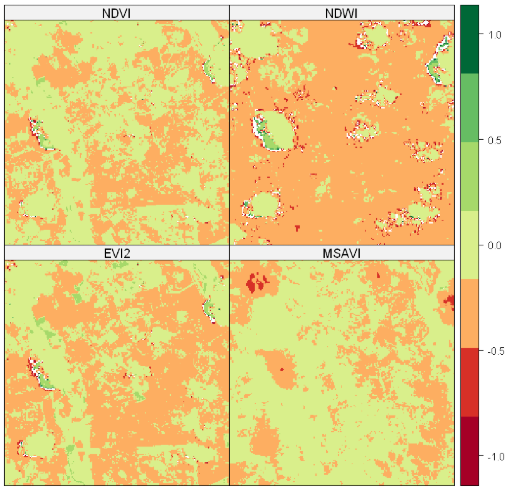
\includegraphics[width=0.97\linewidth]{FIGURAS/indices20131023}
 					\label{fig:ima2013} 
 				\end{figure}			
 				
 			\end{minipage}\hfill
 			\begin{minipage}[t!]{0.31\textwidth}
 				
 				\begin{figure}[H]
 					\centering \small \caption{2016}
 					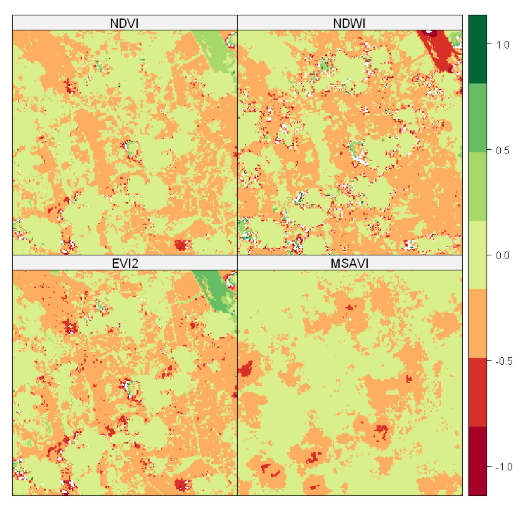
\includegraphics[width=0.97\linewidth]{FIGURAS/indices20160101}
 					\label{fig:inda15} 
 				\end{figure}			
 				
 			\end{minipage} 
 			\begin{minipage}[t!]{0.31\textwidth}
 				
 				\begin{figure}[H]
 					\centering \small \caption{2023}
 					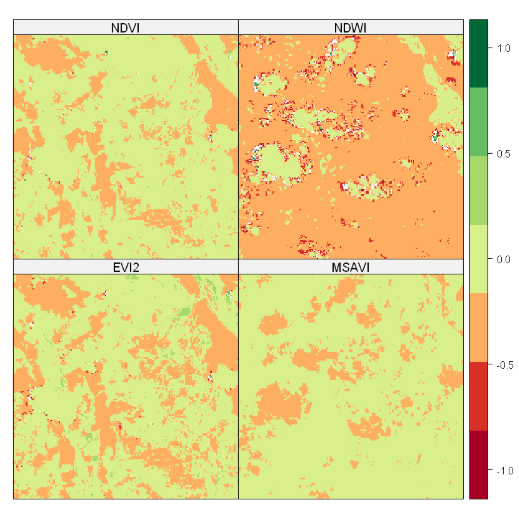
\includegraphics[width=0.97\linewidth]{FIGURAS/indices20231222}
 					\label{fig:inda2023} 
 				\end{figure}		
 			\end{minipage} 
 			
 			\begin{center}
 				Fonte:   Elaborado pelos Autores (2025)
 			\end{center}
 			% }}}
 \hspace*{1.25 cm} Neste conjunto de imagens em nível de cinza,  escolhido a paleta de cores "RdYlGn" do "package ViridisLite" nas Figuras \ref{fig:rplot-ndwi2016} a \ref{fig:difer202332026}, cujas as  medidas pelo sensor e transformadas aos índices espectrais, demonstram que a água ocorreu maior variação neste índice medido e calculado, e por nisso o índice NDWI  foi escolhido para uma análise mais priorizada.   \\
  % {{{   
 			\begin{minipage}[t!]{0.31\textwidth}
 				\begin{figure}[H]
 					\centering \small \caption{NDWI 2016}
 					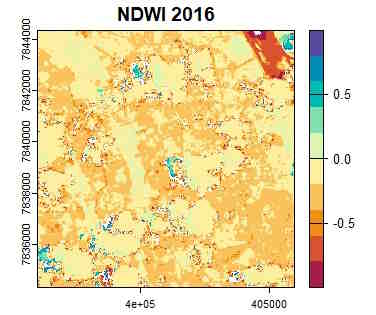
\includegraphics[width=0.97\linewidth]{FIGURAS/Rplotndwi2016}
 					\label{fig:rplot-ndwi2016}
 				\end{figure}			
 				
 			\end{minipage}\hfill
 			\begin{minipage}[t!]{0.31\textwidth}
 				
 				\begin{figure}[H]
 					\centering \small \caption{NDWI 2023}
 					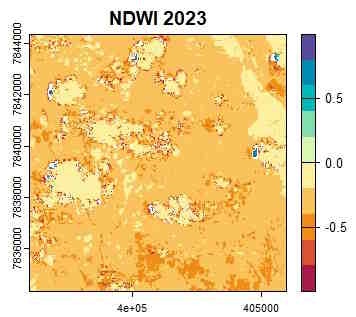
\includegraphics[width=0.97\linewidth]{FIGURAS/Rplot0ndwi2023}
 					\label{fig:rplot0ndwi2023}
 				\end{figure}			
 				
 			\end{minipage} 
 			\begin{minipage}[t!]{0.31\textwidth}
 				
 				\begin{figure}[H]
 					\centering \small \caption{Diferenças no NDWI}
 					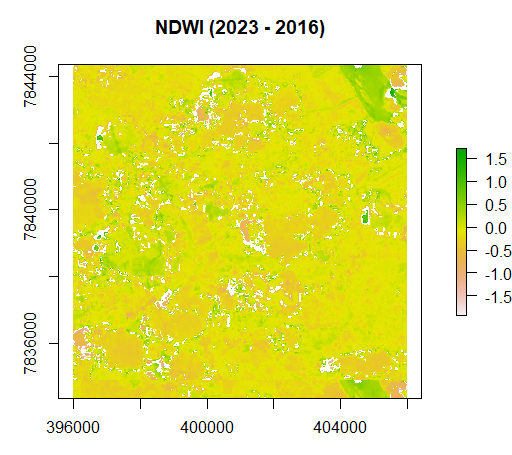
\includegraphics[width=0.97\linewidth]{FIGURAS/difer202332026}
 					\label{fig:difer202332026}
 				\end{figure}		
 			\end{minipage} 
 			
 			\begin{center}
 				Fonte:   Elaborado pelos Autores (2025)
 			\end{center}
 			% }}}		
	%	
 \hspace*{1.25 cm}  Ao destacarmos o índice NDWI nas duas imagens com diferença temporal de 8(oito)anos, temos a Figura   \ref{fig:difer202332026} e nesta a atenção pode ser observada no canto superior direito, e em outras superfícies com maior presença de água, como brejos e açudes, a alteração contrastante destas diferenças.  \\
 %------------------
  \begin{wrapfigure}{r}{0.65\textwidth}
	\begin{center}
		\centering  \small \caption{Amostragem em grid}
		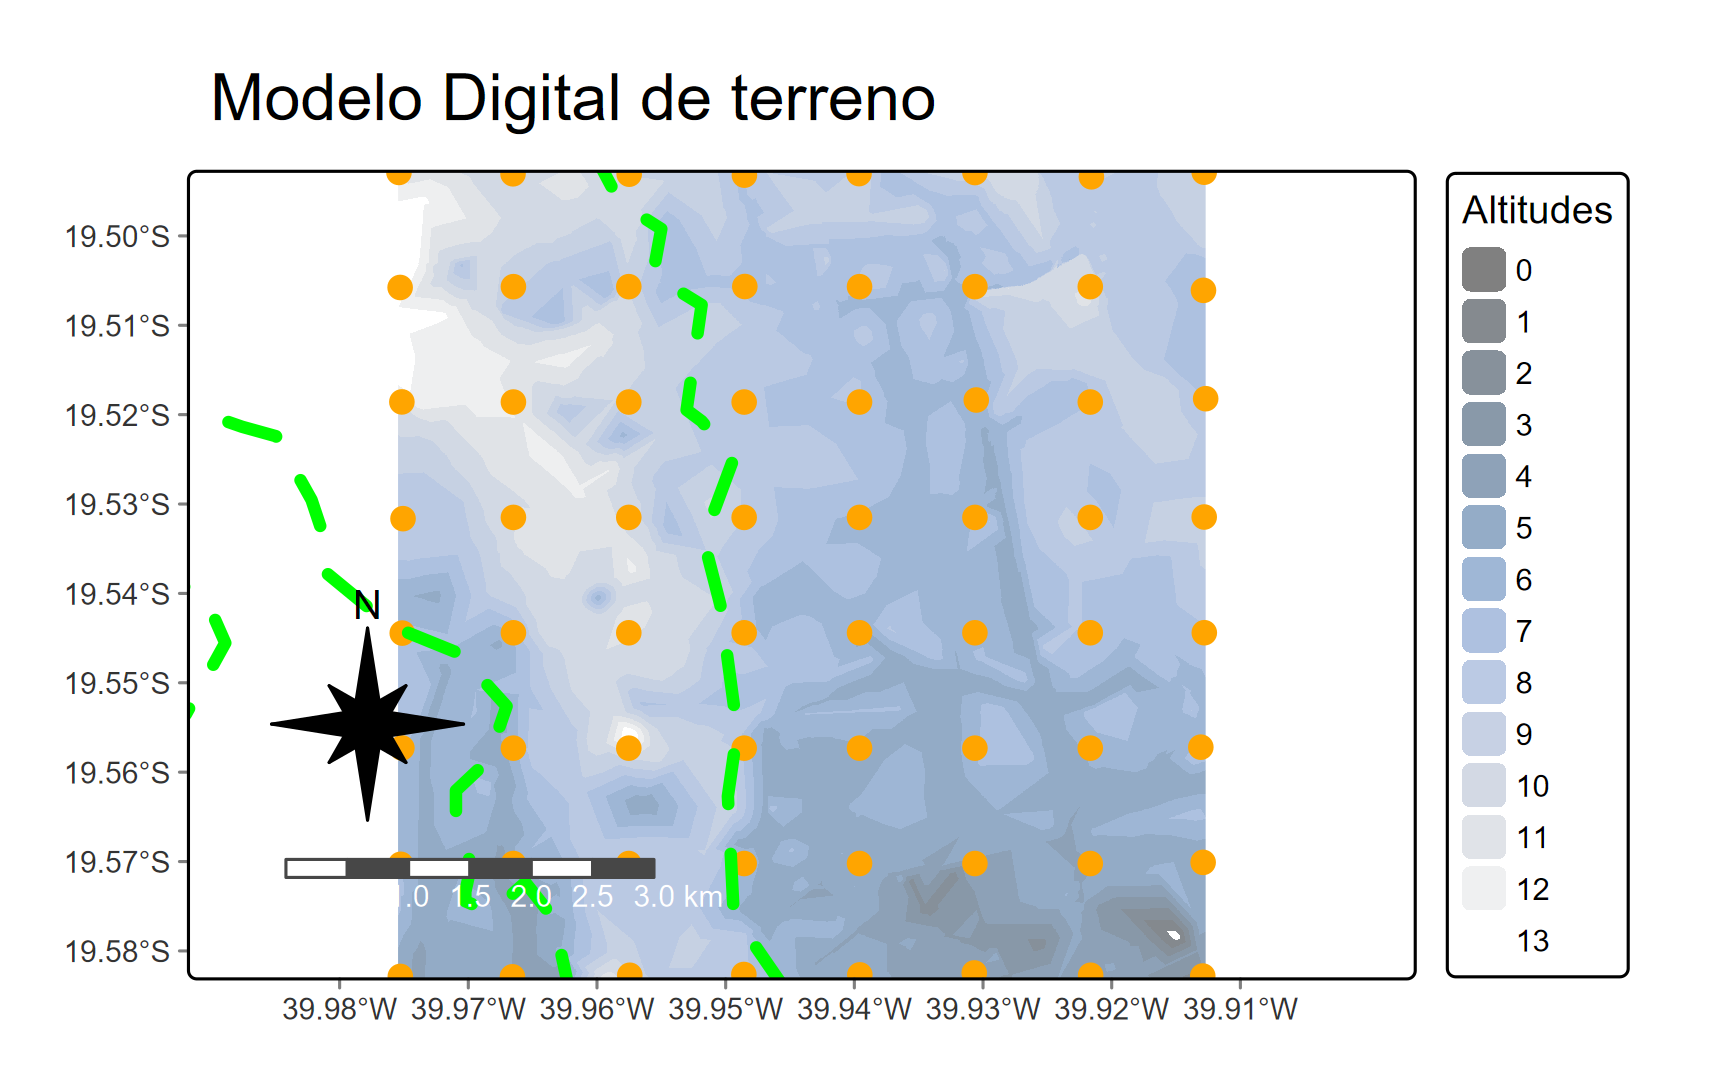
\includegraphics[width=0.97\linewidth]{FIGURAS/mdtamostras}
		\label{fig:mdtamostras}\\{ Fonte:   Elaborado pelos Autores (2025)}
	\end{center}
\end{wrapfigure} 
\subsection{Geoestátistica}
 %------------------
  \hspace*{1.25 cm}  Neste momento, a percepção do objeto observado ser uma superfície, quase continua(excluídos vazios radiométricos), torna-se inerente ao fenômeno de estudo. E por ser uma superfície, com valores máximos, mínimos, direção, desvio padrão e variância do valor do índice com coordenada (x,y). Deve ser tratada como tal, e ser analisadas  por técnicas da geoestátistica.   \\
  %------------------
  \hspace*{1.25 cm}  Ao decimo sétimo e oitavo paragrafo da seção 3, ao descrevermos a estrutura de amostragem, e ao parágrafo anterior  que  compreendemos a estrutura do fenômeno com uma \underline{variável regionalizada}, e por isso voltamos a  \cite[p.10]{Yamamoto} :
\begin{quoting}[rightmargin=0cm,leftmargin=4cm]
	\begin{singlespace}
		{
			\textit{Os métodos geoestatísticos fornecem um conjunto de técnicas necessárias para entender a aparente aleatoriedade dos dados, os quais apresentam, porém, uma possível estruturação espacial, estabelecendo, desse modo, uma função de correlação espacial.}
		}
	\end{singlespace}
\end{quoting} 
 %------------------
 \hspace*{1.25 cm} Ainda em  \cite[p.19 e 20]{Yamamoto}, o fenômeno estudado se comporta dentro de domínios, sejam em 2D ou 3D, e apresentam distribuição e variabilidade espaciais. A "metodologia da geoestátistica se destaca ao oferecer a incerteza associada à estimativa" \\
 %
  \hspace*{1.25 cm} Continuando em  \cite[p.20 e 21]{Yamamoto}, na "\textit{reprodução das característica do fenômeno espacial baseado em pontos amostrais é denominado interpolação ou estimativa}". O processo de para inferir a distribuição e a variabilidade espacial, vai  depender do tamanho da amostra e da distribuição espacial, e em nosso caso se estabeleceu tanto por aleatoriedade Figura \ref{fig:usoSOLOamostras} e Figura \ref{fig:mdtamostras} \\
 %
  \hspace*{1.25 cm}  Coletado os dados, e tabulados, necessitamos fazer a sumarização e analise exploratória,  no entanto varias vezes verificamos  situações que impossibilita termos conclusões sobre os seus resultados. E como em  \cite[p.18]{Webster}, muitas variáveis ambientais, principalmente nas  concentradas no solo, estão na forma de distribuição normal, de acordo com as "\textit{descoberta independentemente por De Moivre, Laplace e Gauss, mas Gauss parece geralmente levar o crédito por ela. E a distribuição é frequentemente chamada de "gaussiana"}". \\
%
  \hspace*{1.25 cm}  Ainda em \cite[p.20]{Webster}, mas a utilização destes dados na formulação de modelos, apresentam dificuldades, podemos transformar os valores medidos a uma nova escala, "\textit{se necessário, transformar os resultados para a escala original ao final}." \\
 % 
\hspace*{1.25 cm}  Na Figura \ref{fig:difer202332026} realizando operações de interpolação com a utilização do grid, conseguimos obter uma imagem com alguma normalidade, Figura \ref{fig:RplotN16}. No entanto ao aplicarmos o \textbf{\textcolor{blue}{bestnormalize}}, os resultado é surpreendente, tanto que apresentamos em Figura \ref{fig:RplotMELNHOR}, e nos estimulou a geração do modelo matemático em 3D, Figura \ref{fig:RplotP34}\\
%---------------- 
  % {{{   
 			\begin{minipage}[t!]{0.31\textwidth}
 				\begin{figure}[H]
 					\centering \small \caption{Antes da normalização}
 					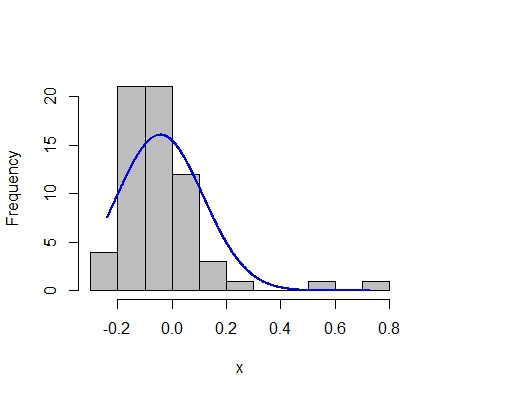
\includegraphics[width=0.97\linewidth]{FIGURAS/RplotN1}
 					\label{fig:RplotN16}
 				\end{figure}			
 				
 			\end{minipage}\hfill
 			\begin{minipage}[t!]{0.31\textwidth}
 				
 				\begin{figure}[H]
 					\centering \small \caption{Apôs a normalização}
 					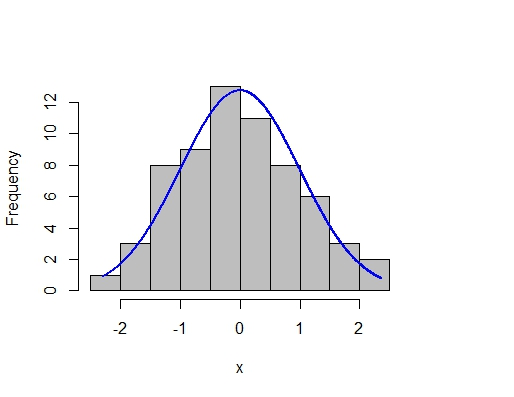
\includegraphics[width=0.97\linewidth]{FIGURAS/RplotMELNHOR}
 					\label{fig:RplotMELNHOR}
 				\end{figure}			
 				
 			\end{minipage} 
 			\begin{minipage}[t!]{0.31\textwidth}
 				
 				\begin{figure}[H]
 					\centering \small \caption{Perspectiva da Superfície}
 					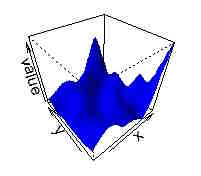
\includegraphics[width=0.97\linewidth]{FIGURAS/RplotP34}
 					\label{fig:RplotP34}
 				\end{figure}		
 			\end{minipage} 
 			
 			\begin{center}
 				Fonte:   Elaborado pelos Autores (2025)
 			\end{center}
 			% }}}
 %%--------------
 \lstset{
	language=R, % Define a linguagem como JavaScript
	caption= Sujestões de melhoria ao modelo em  linguagem R} % Legenda do código
\begin{lstlisting}[language=R]
 Best Normalizing transformation with 64 Observations
Estimated Normality Statistics (Pearson P / df, lower => more normal):
- arcsinh(x): 1.7857
- Center+scale: 1.8024
- Double Reversed Log_b(x+a): 1.7667
- Exp(x): 1.9929
- Log_b(x+a): 1.5042
- orderNorm (ORQ): 1.4643
- sqrt(x + a): 1.2955
- Yeo-Johnson: 1.2452
Estimation method: Out-of-sample via CV with 10 folds and 5 repeats 
Based off these, bestNormalize chose:
Standardized Yeo-Johnson Transformation with 64 nonmissing obs.:
Estimated statistics:
- lambda = -3.643204 
- mean (before standardization) = -0.09376124 
- sd (before standardization) = 0.1402468
\end{lstlisting}  
% 
\hspace*{1.25 cm} A produção inicial do variograma,  com procedimentos em \cite[p.224]{Bivand}, com a caracterização mensurada e sua distância em visão inicial da análise em Figura \ref{fig:variinical}\\
 %%%===================
 \begin{minipage}[t!]{0.5\textwidth}
 	\begin{figure}[H]
 		\centering \small \caption{Semivariograma sem definição do modelo explicativo}
 		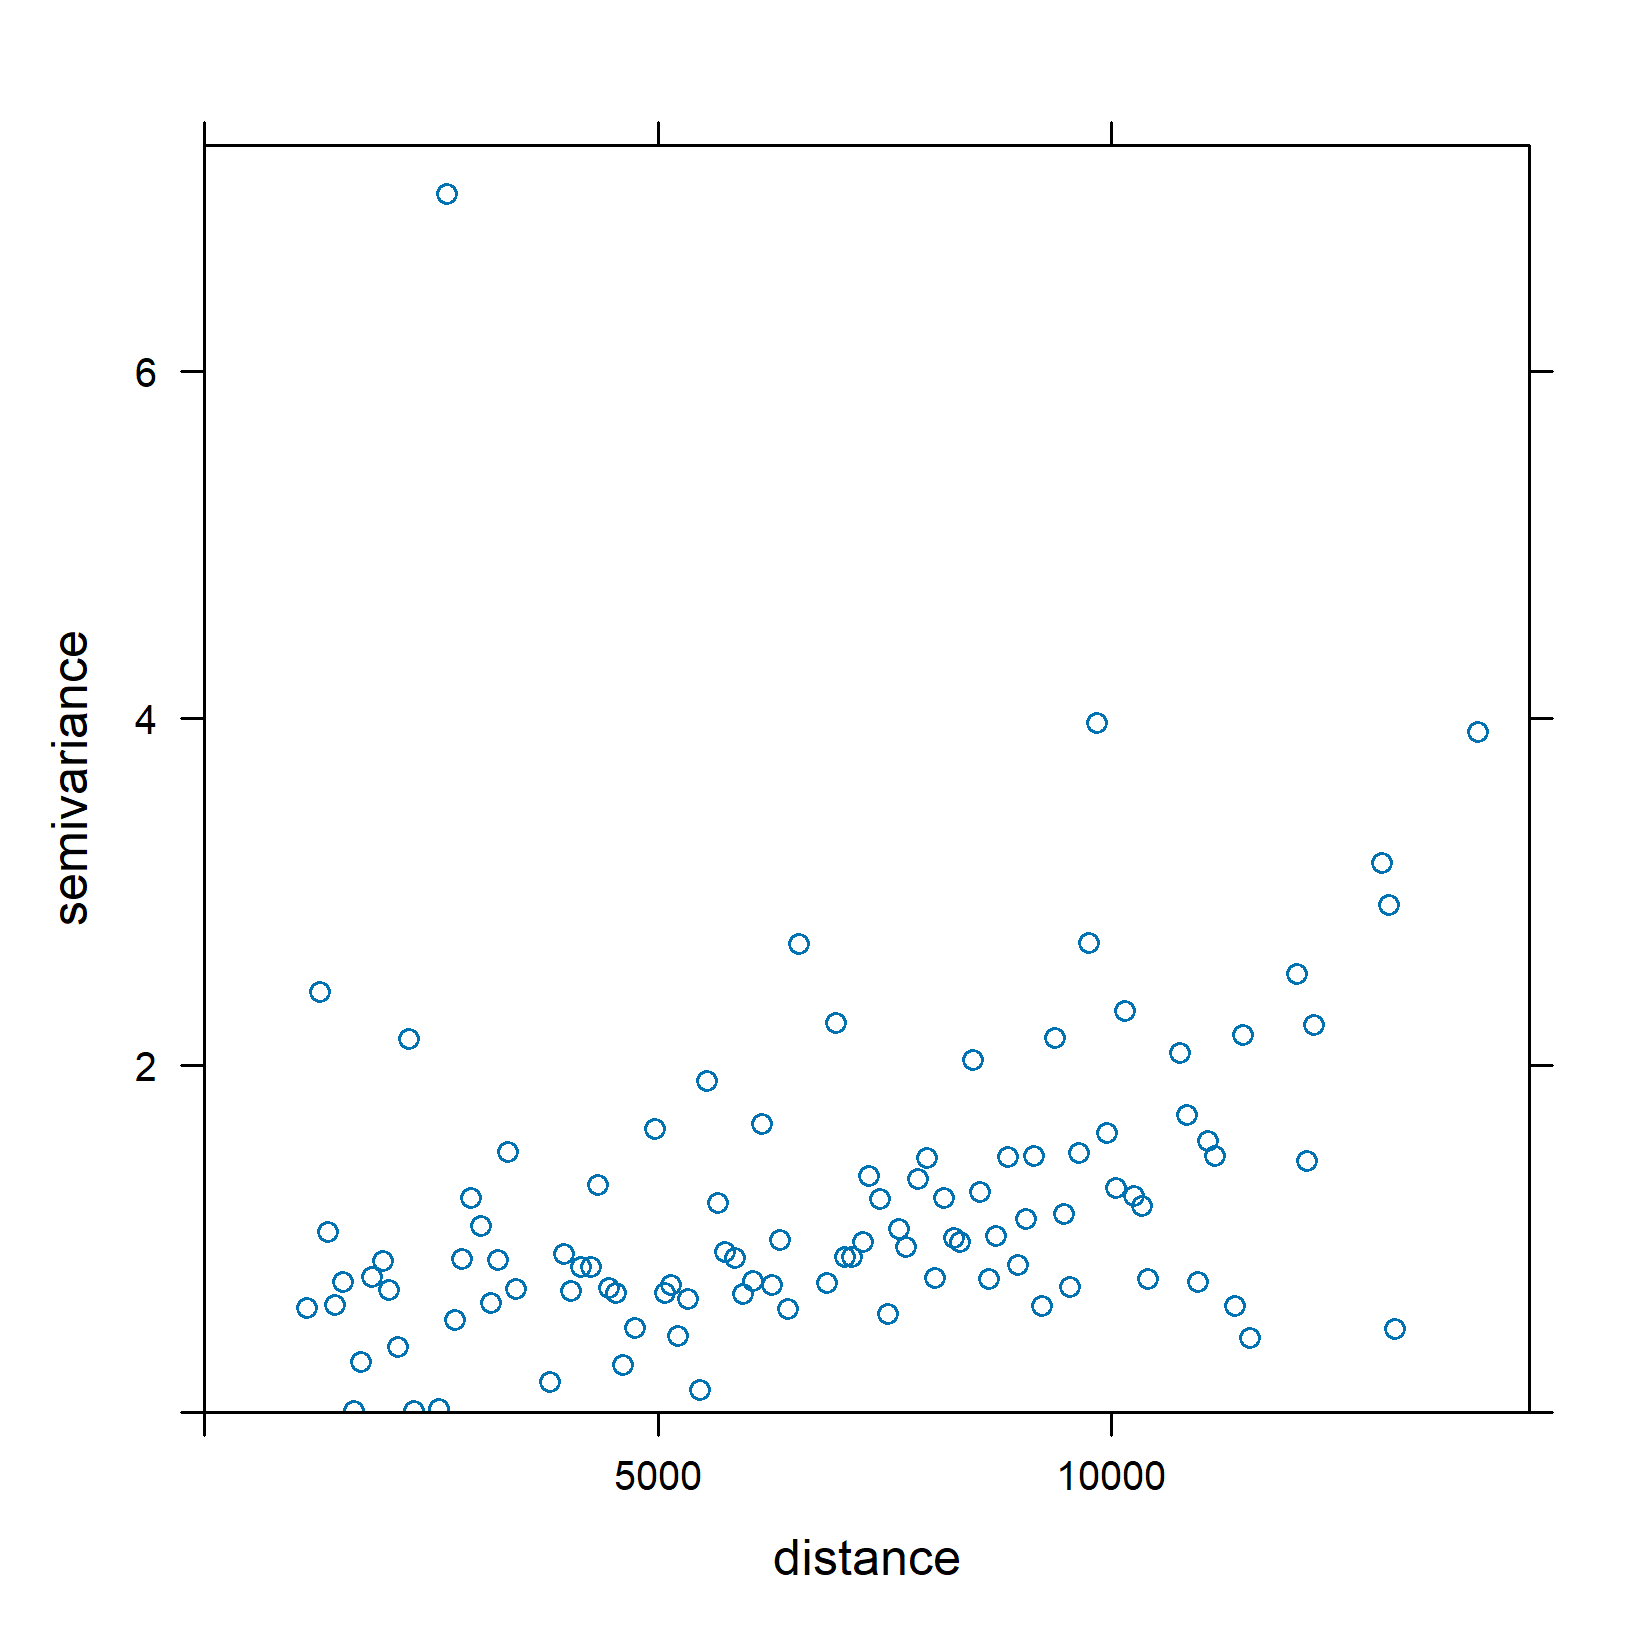
\includegraphics[width=0.97\linewidth]{FIGURAS/variogramaPTONOS}
 		\label{fig:variinical}
 	\end{figure}	
 \end{minipage}\hfill
 \begin{minipage}[t!]{0.5\textwidth}
 	\begin{figure}[H]
 		\centering \small \caption{Modularização da reflectância}
 		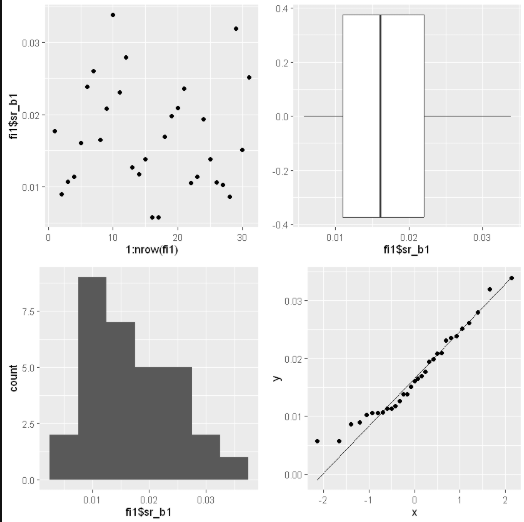
\includegraphics[width=0.97\linewidth]{FIGURAS/normali}
 		\label{fig:Rplothdg}
 	\end{figure}		
 \end{minipage} 
 % {{{   			
 			\begin{center}
 				Fonte:   Elaborado pelos Autores (2025)
 			\end{center}
 			% }}
 %==========================================		
%\hspace*{1.25 cm} E seu modelo de superfície plana, pode ser apreciado em Figura \ref{fig:superficie} critérios que podem também ser observados em Figura \ref{fig:superficie1} e sua melhora e Figura  \ref{fig:Rplothdg}\\
 		 %%-------------- 
  \hspace*{1.25 cm} A escolha da função matemática que produza, e nos possibilite a explicar o modelo, pode ser encontrada em  \cite[p.90]{delgado}, e a mesma deve ser inserido os parâmetros e efeitos, com o significado em língua inglesa que são o patamar ("sill"), pepita("nugget"), comprimento("range") e sua contribuição("contribution") .	\\	
 		 %%-------------- 
% {{{   
			\begin{minipage}[t!]{0.31\textwidth}
				\begin{figure}[H]
					\centering \small \caption{ Escolha da função }
					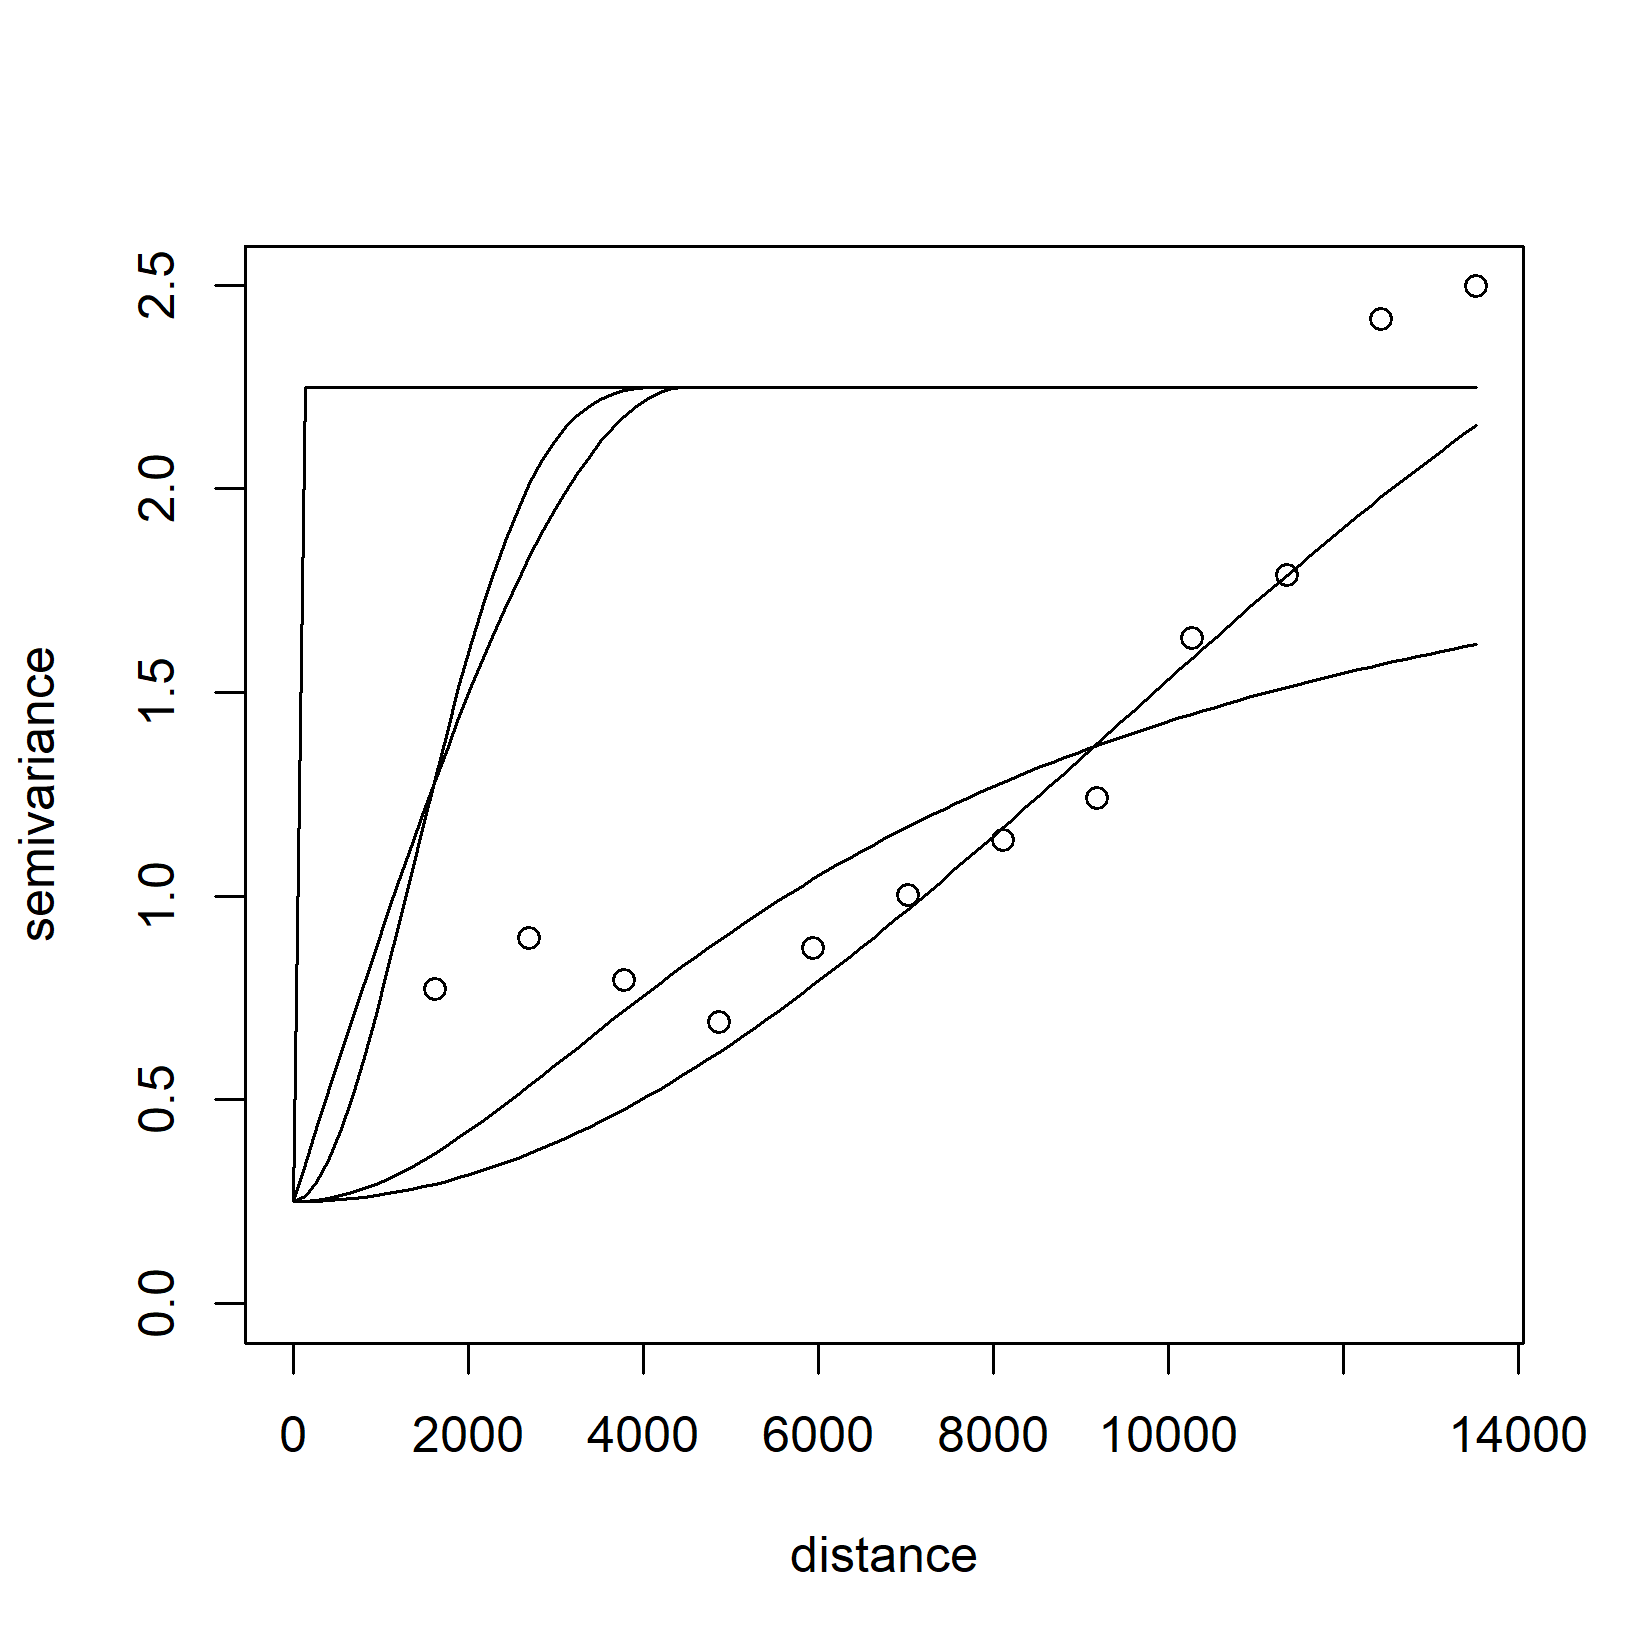
\includegraphics[width=0.97\linewidth]{FIGURAS/variogramageor4}
					\label{fig:variogramageor4}
				\end{figure}			
				
			\end{minipage}\hfill
			\begin{minipage}[t!]{0.31\textwidth}
				
				\begin{figure}[H]
					\centering \small \caption{Modelo esférico}
					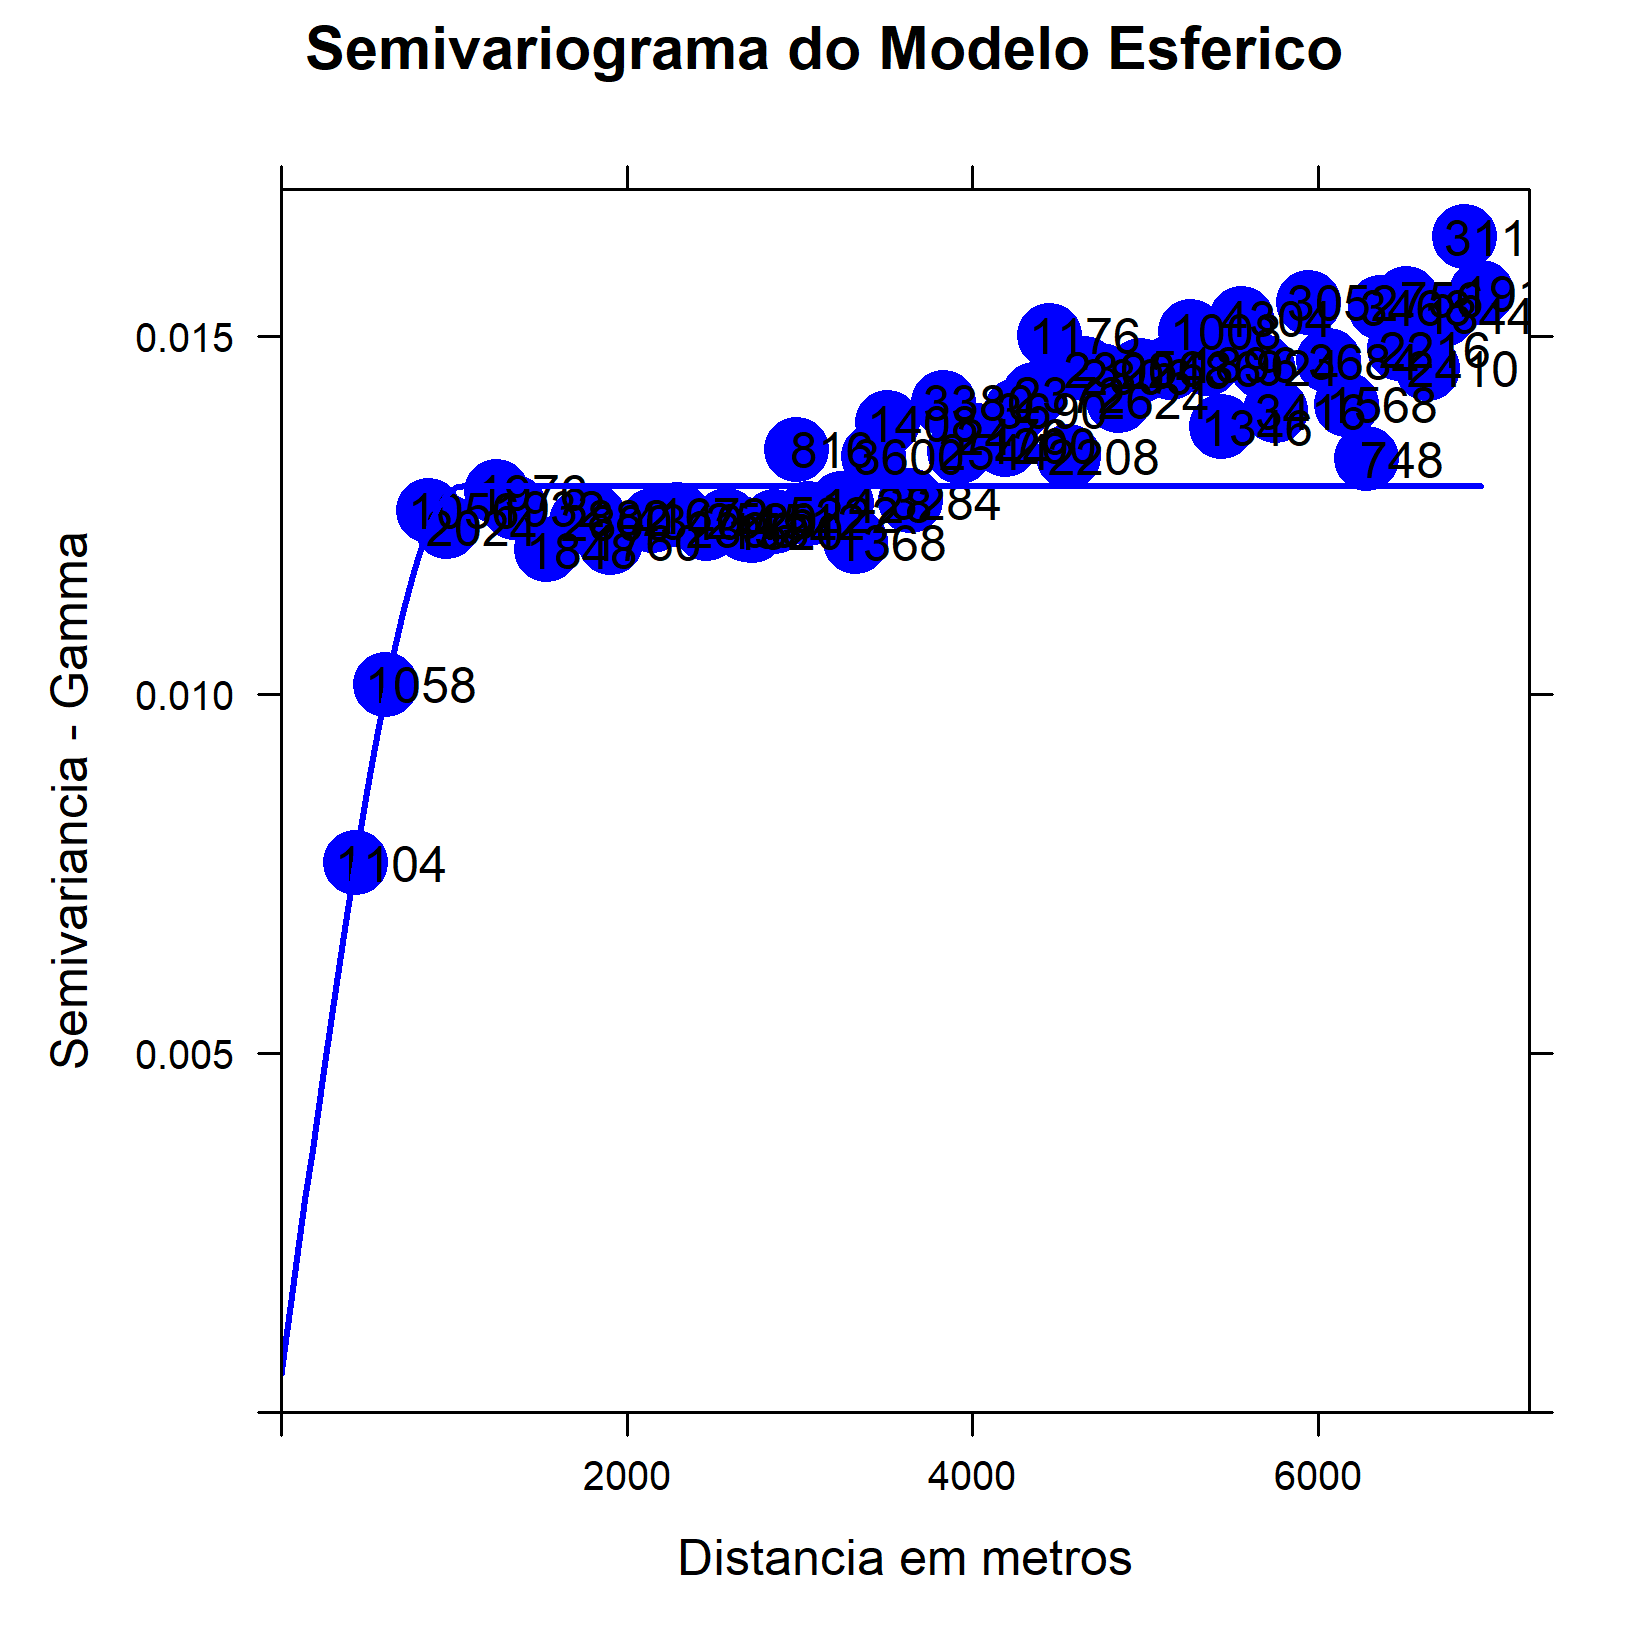
\includegraphics[width=0.97\linewidth]{FIGURAS/modelos-esferico}
					\label{fig:varexpfitsp}
				\end{figure}			
				
			\end{minipage} 
			\begin{minipage}[t!]{0.31\textwidth}
				
				\begin{figure}[H]
					\centering \small \caption{Validação cruzada}
					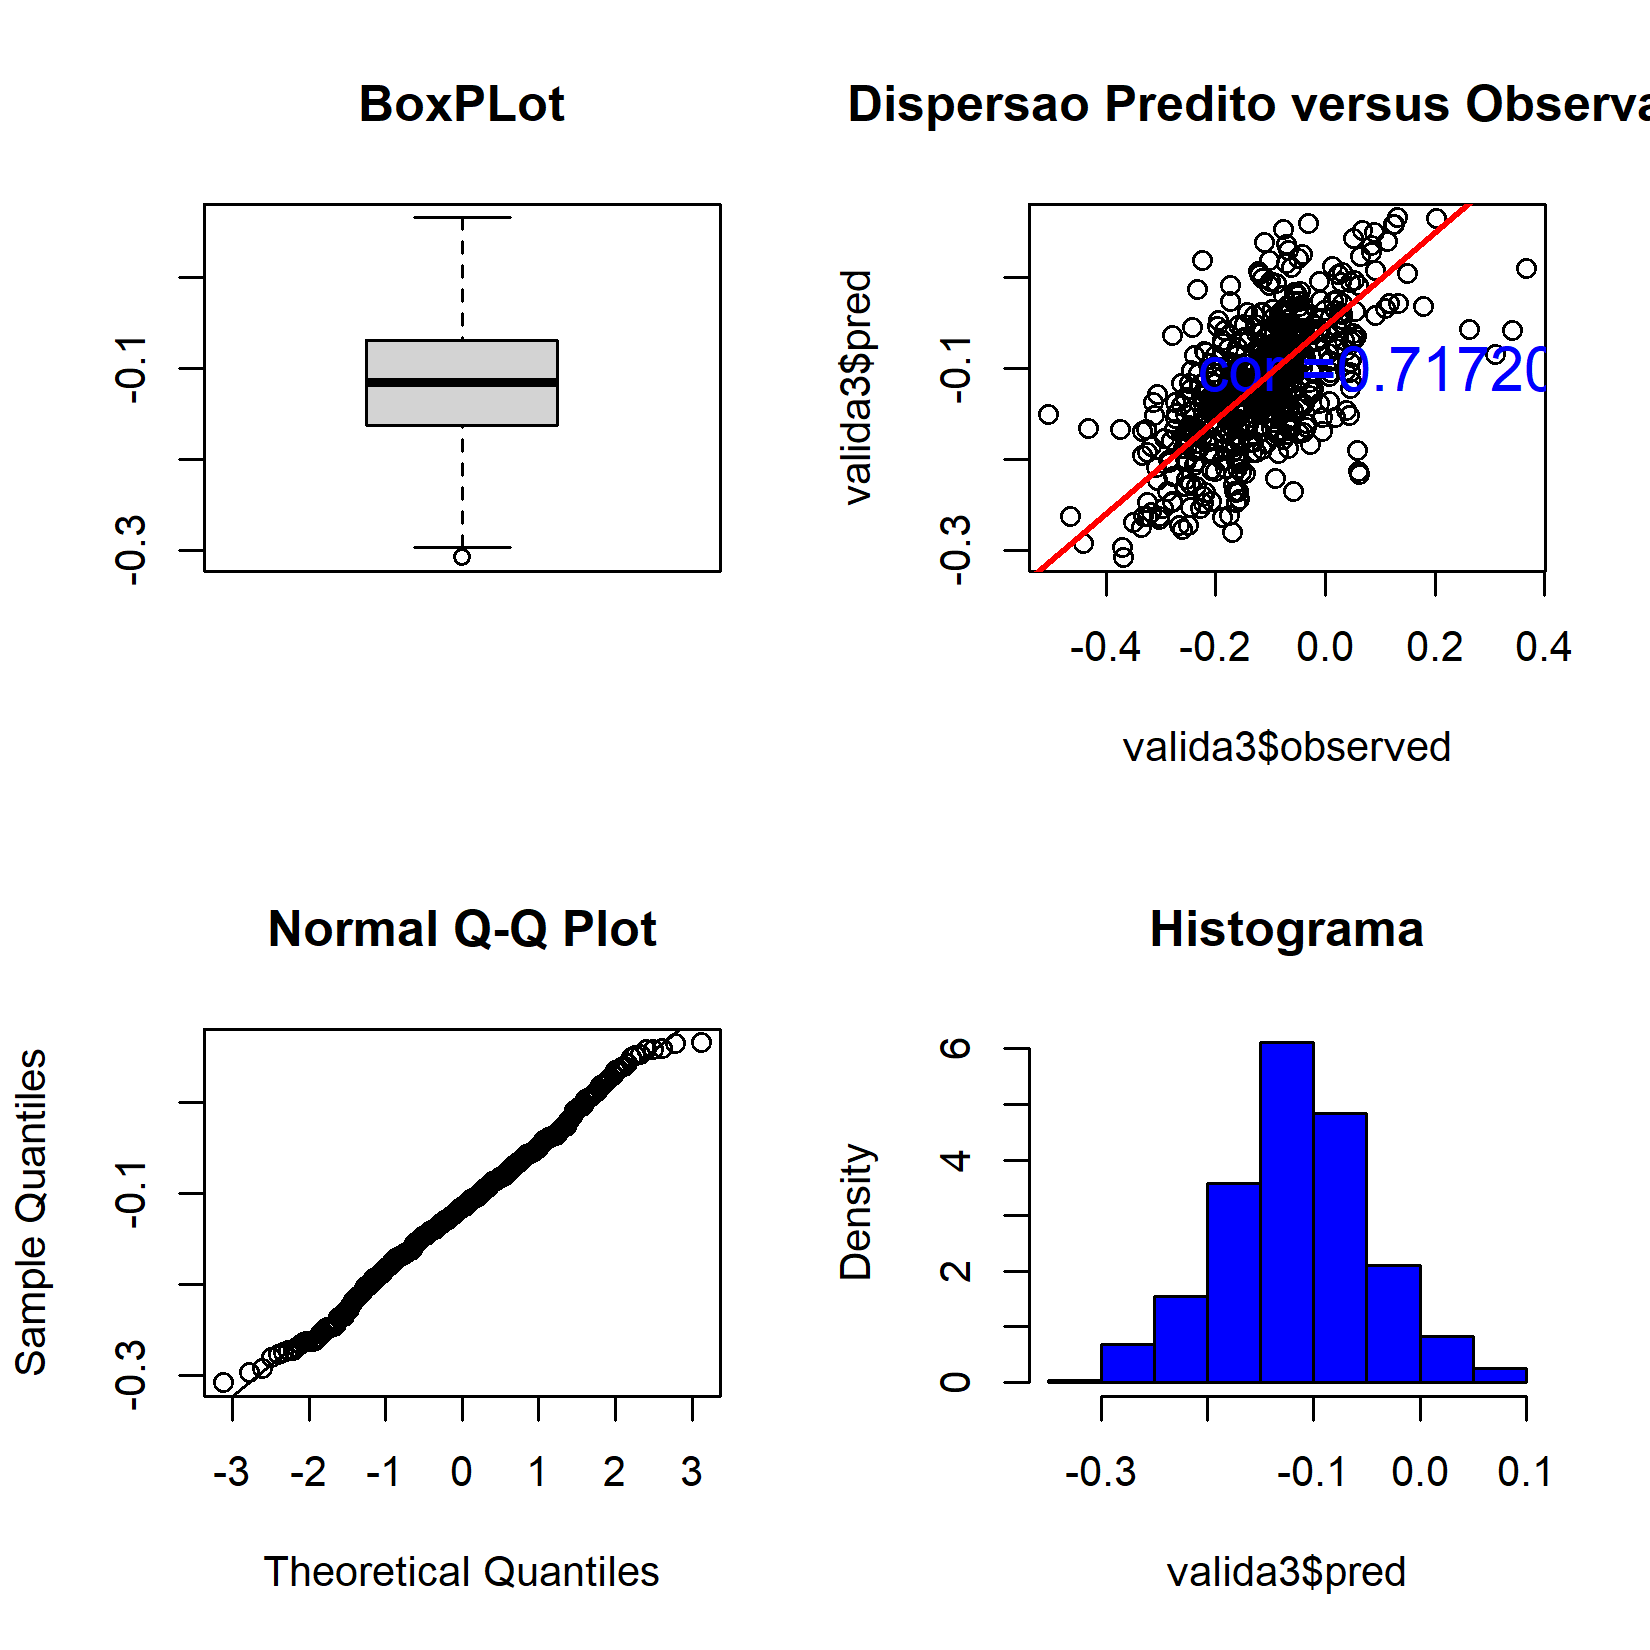
\includegraphics[width=0.97\linewidth]{FIGURAS/valicas}
					\label{fig:xvalid.cruzadaesferica2}
				\end{figure}		
			\end{minipage} 
			
			\begin{center}
				Fonte:   Elaborado pelos Autores (2025)
			\end{center}
			% }}
 \hspace*{1.25 cm} 	Em todas as Figuras \ref{fig:variinical} e \ref{fig:superfdicie} que a estacionáriedade  inicia-se visualmente em aproximadamente em 0,9 e seu "range" em torno de 1300 metros\\
 %		
 \hspace*{1.25 cm} Na Figura \ref{fig:variogramageor4} o processo da escolha da função, na Figura \ref{fig:varexpfitsp} a função escolhida, e finalmente na Figura \ref{fig:xvalid.cruzadaesferica2} a validação cruzada, com a regressão em homocedasticidade\\
 %%-------------- 
 \hspace*{1.25 cm} Em Figura \ref{fig:superfdicie}, temos a superfície da interpolação, com a analise da covariância do modelo, distribuído espacialmente em Figura \ref{fig:htrrtyR} , com procedimentos vistos em   \cite[p.47]{delgado}, e como cada variável, seus resíduos, e observação contribuem na explicação do modelo em \ref{fig:Rplothddg} \\
   % {{{   
 			\begin{minipage}[t!]{0.31\textwidth}
 				\begin{figure}[H]
 					\centering \small \caption{Superfície interpolada}
 					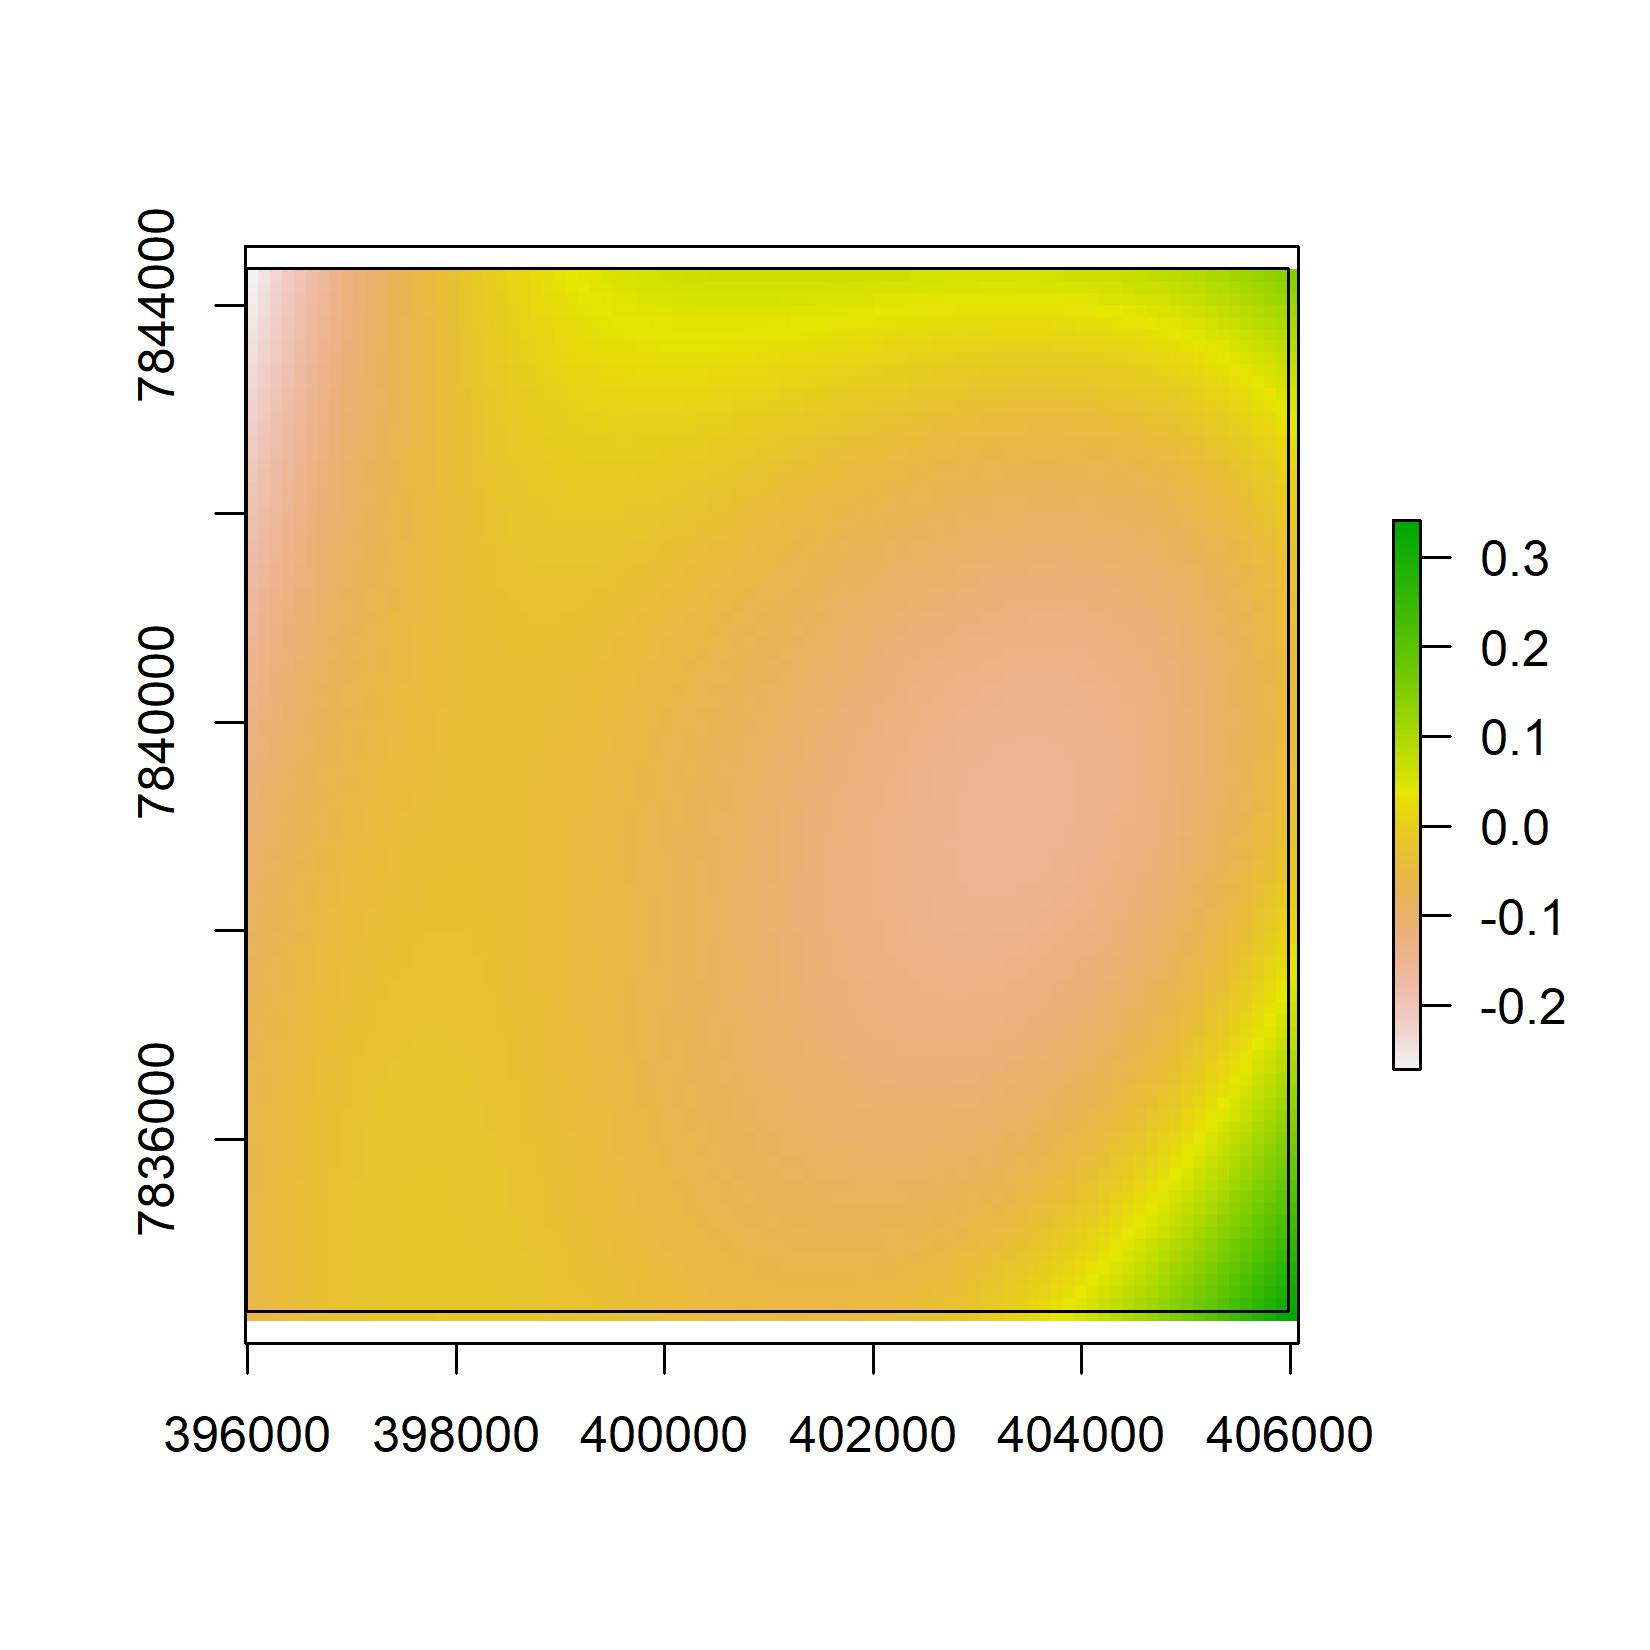
\includegraphics[width=0.97\linewidth]{FIGURAS/superficie}
 					\label{fig:superfdicie}
 				\end{figure}			
 				
 			\end{minipage}\hfill
 			\begin{minipage}[t!]{0.31\textwidth}
 				
 				\begin{figure}[H]
 					\centering \small \caption{Modelo esférico}
 					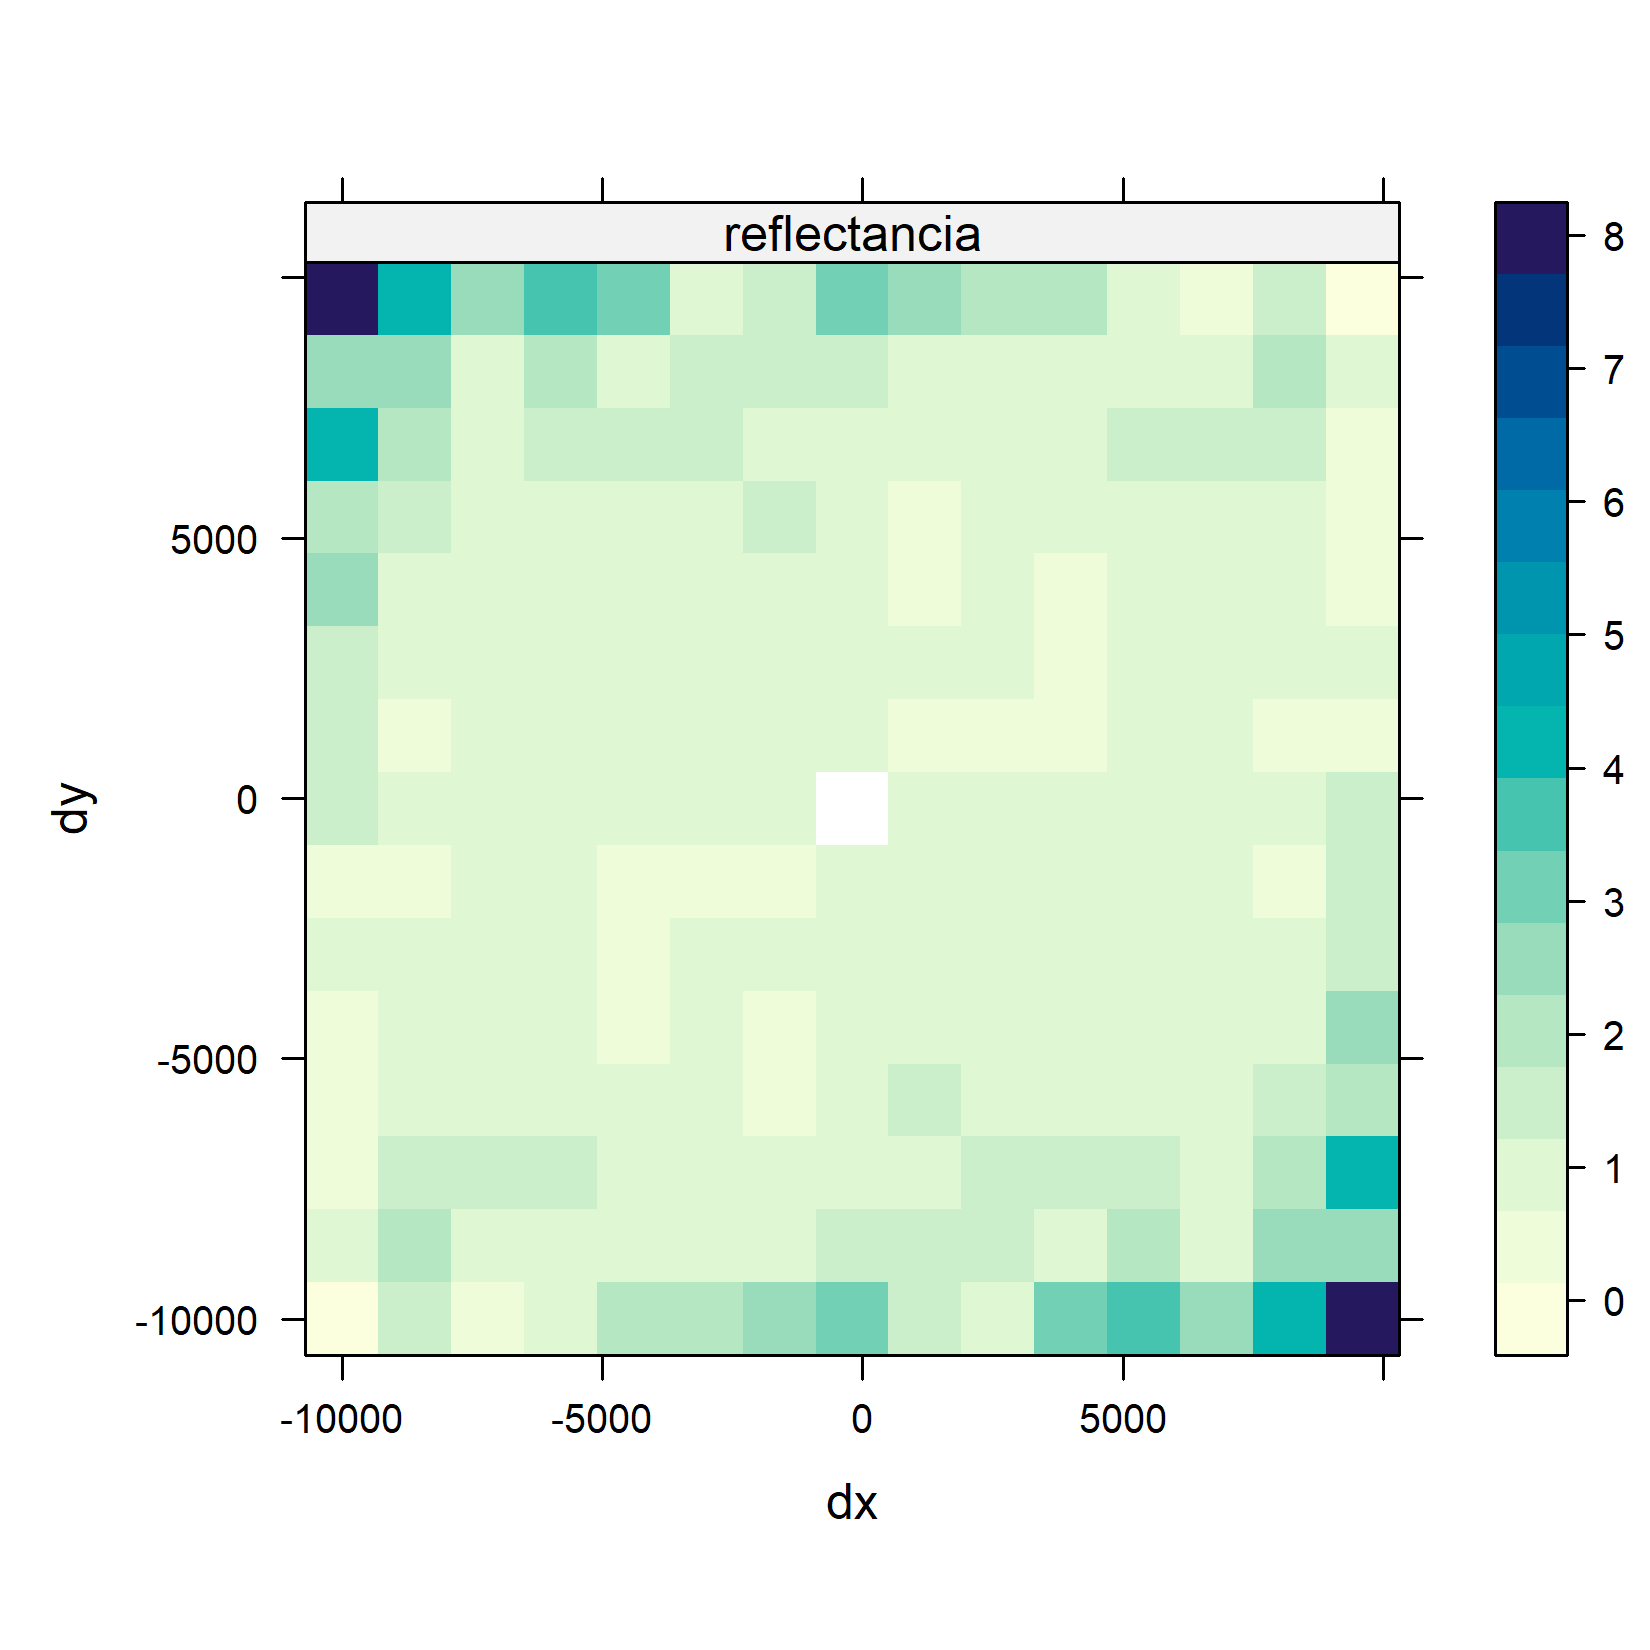
\includegraphics[width=0.97\linewidth]{FIGURAS/varexpmap}
 					\label{fig:htrrtyR}
 				\end{figure}			
 				
 			\end{minipage} 
 			\begin{minipage}[t!]{0.31\textwidth}
 				
 				\begin{figure}[H]
 					\centering \small \caption{Contribuição espacial das variável mensurada}
 					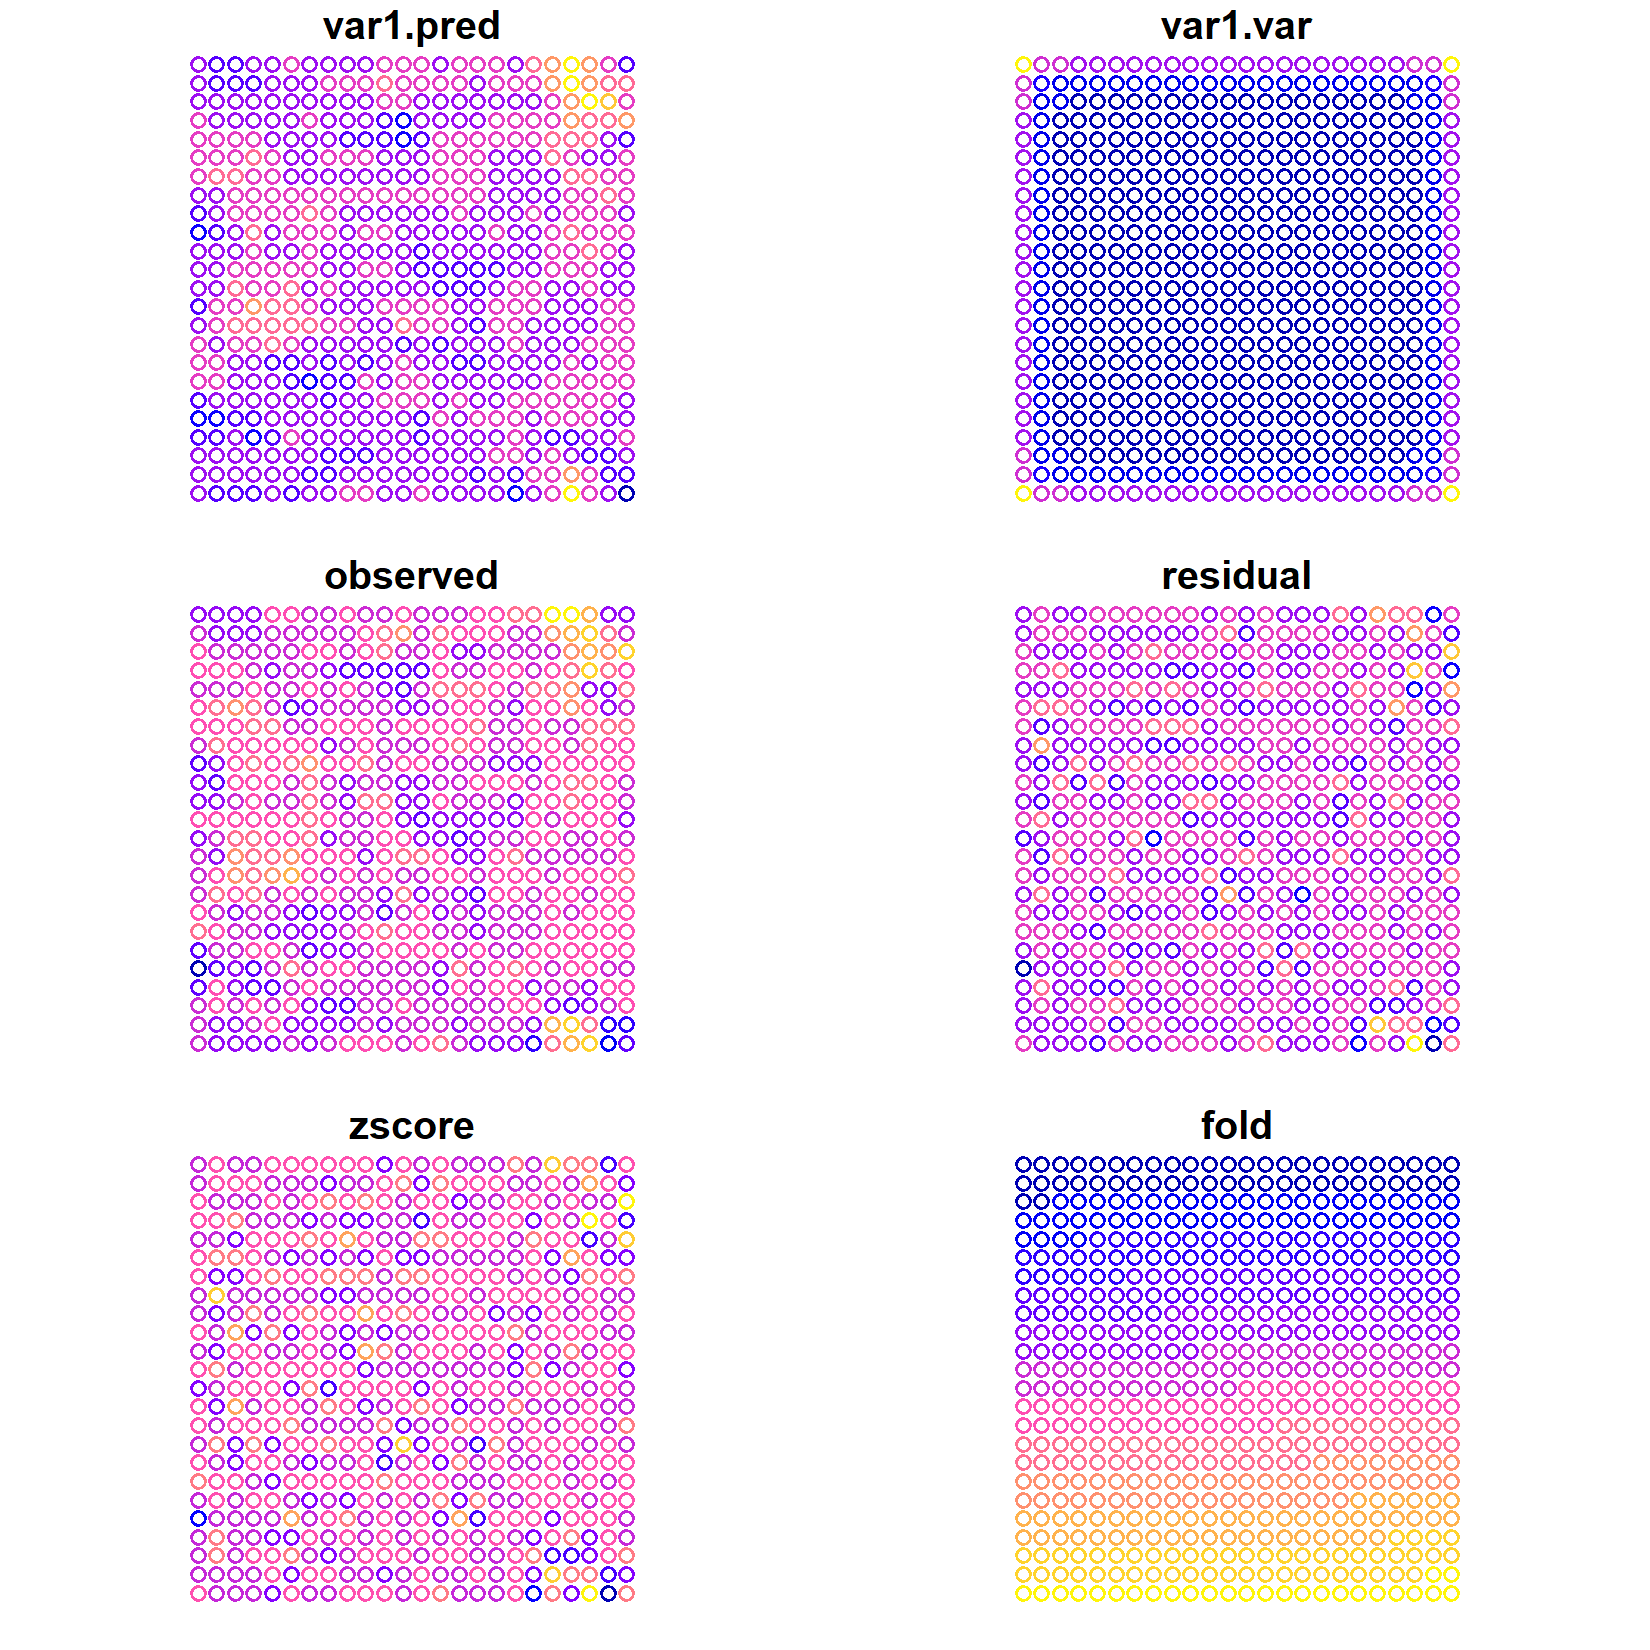
\includegraphics[width=0.97\linewidth]{FIGURAS/xvalid.sph-map}
 					\label{fig:Rplothddg}
 				\end{figure}		
 			\end{minipage} 
 			
 			\begin{center}
 				Fonte:   Elaborado pelos Autores (2025)
 			\end{center}
 			% }}

\hspace*{1.25 cm} Dando o enfoque no modelo esférico,  determinados enfase nos parâmetros deste modelo. E passo que escolhemos o modelo, sendo que o resultado erro médio quadrático  e a porcentagem explicada do modelo em quadra a seguir. 
%%
\lstset{
	language=R, % Define a linguagem como R
	caption= Resultado do modelo de superficie de tendencia de 3 grau saida da linguagem R} % Legenda do código
\begin{lstlisting}[language=R]
.0364868216565002  # root mean squared error
A matrix: 1 × 1 of type dbl
0.9465385  # % de explicacao do modelo
\end{lstlisting}   
 	\begin{figure}[H]
	\centering  \small \caption{Modelagem por krigagem}
	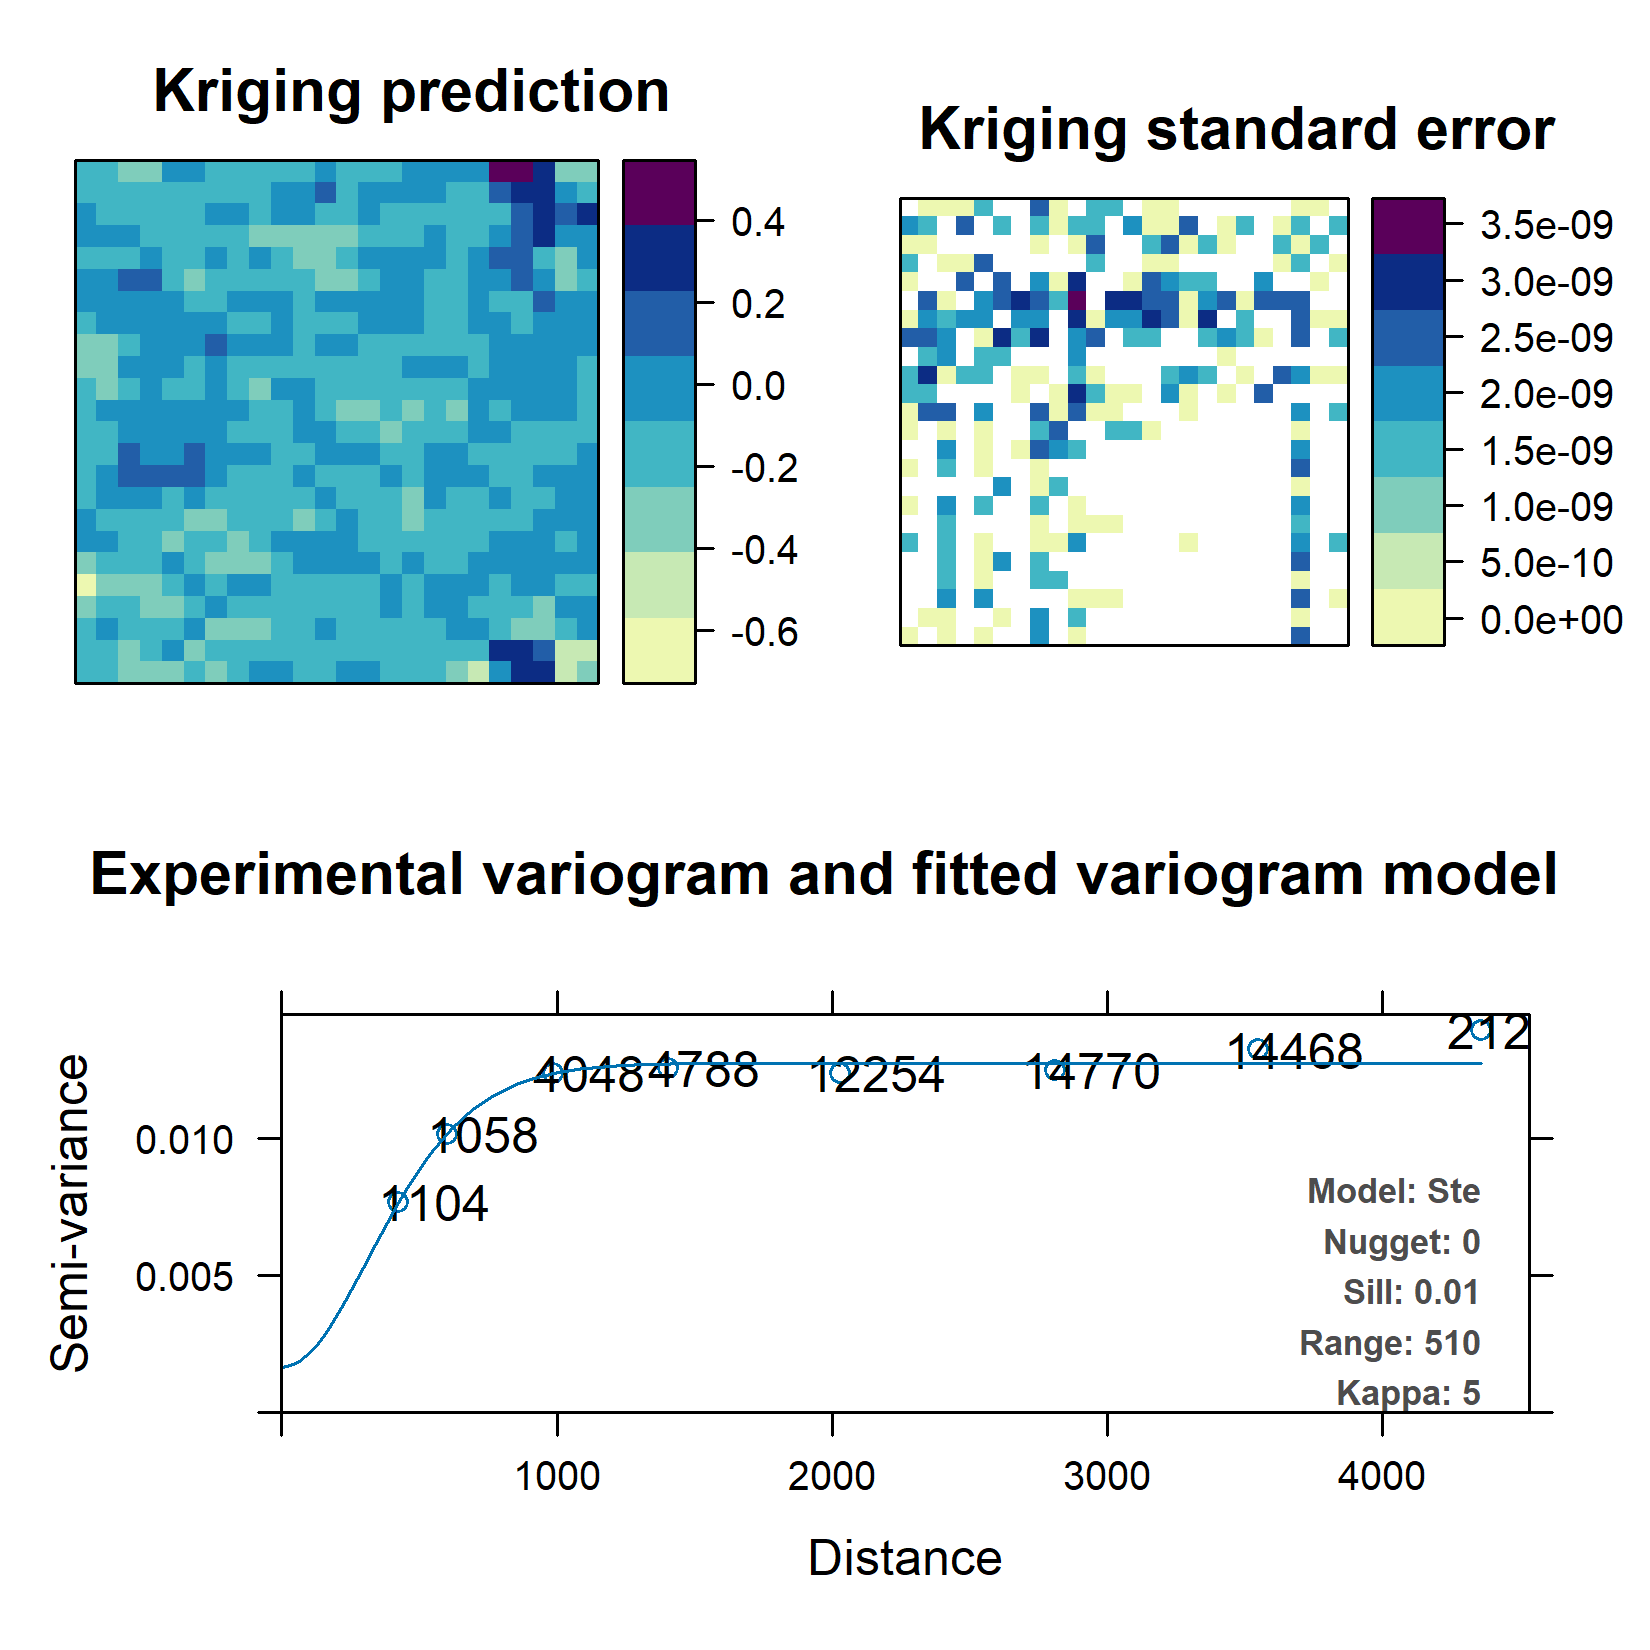
\includegraphics[width=0.57\linewidth]{FIGURAS/MODELOKRIGAGEM-MELHOR}
	\label{fig:rplotkriga}\\{ Fonte:   Elaborado pelos Autores (2025)}
\end{figure}


 \begin{comment}
 	  \begin{wrapfigure}{l}{0.506\textwidth}
 		\begin{center}
 			\centering  \small \caption{Modelagem por krigagem}
 			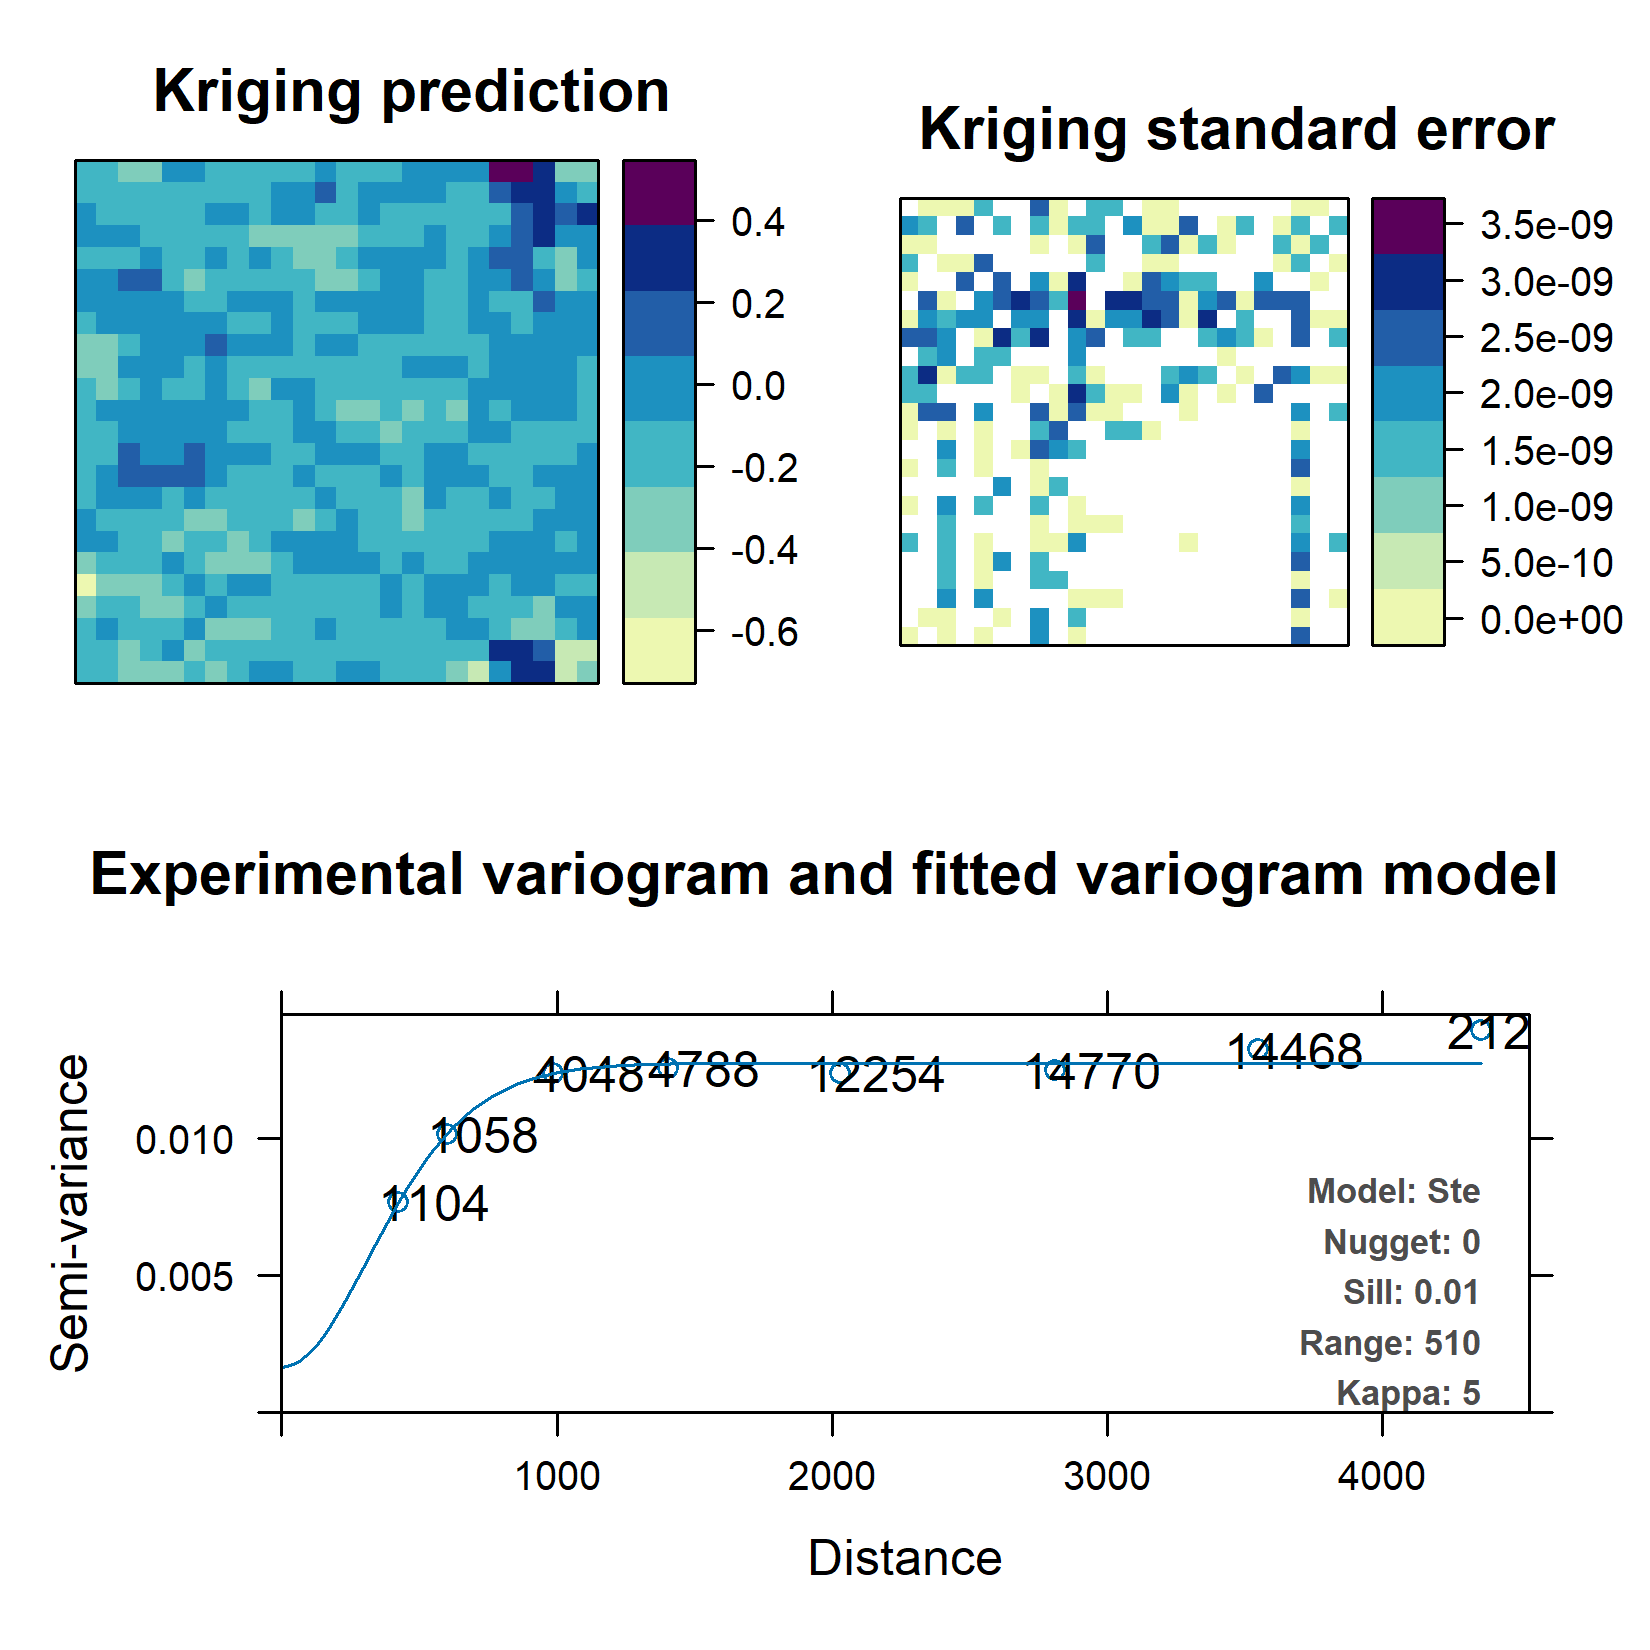
\includegraphics[width=0.97\linewidth]{FIGURAS/MODELOKRIGAGEM-MELHOR}
 			\label{fig:rplotkriga}\\{ Fonte:   Elaborado pelos Autores (2025)}
 		\end{center}
 	\end{wrapfigure} 	 
 	

 	
 	%%%%%%%%%%%%%%%%%%%%%%%%%%%%%%%%%%%

 \end{comment}
  
\hspace*{1.25 cm} O que nos animou a elaboração da krigagem em Figura \ref{fig:rplotkriga}, o que possibilita ao lado direito da figura os locais onde ocorrem os maiores erros, na determinação desta superfície. E para também o variograma ficou próximo ao da Figura \ref{fig:Rplothddg}  \\
 
 \begin{comment}
\begin{figure}
	\centering
	\caption{}
	\label{fig:rplotndwi2016}
	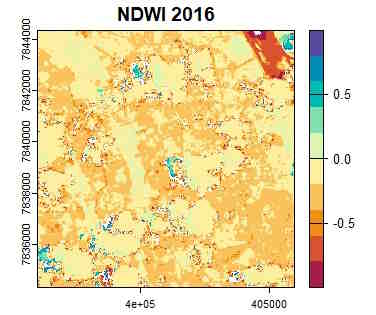
\includegraphics[width=0.97\linewidth]{FIGURAS/Rplotndwi2016}
\end{figure}
 	\begin{center}
 		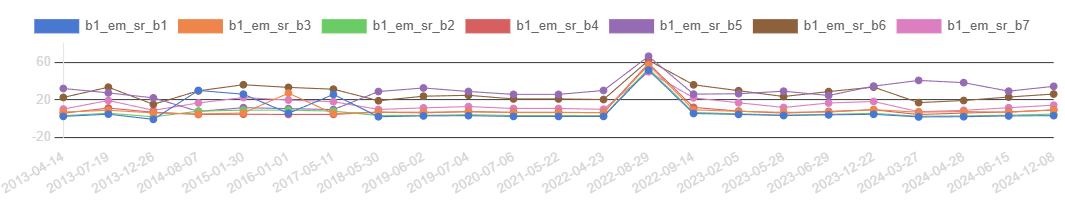
\includegraphics[width=0.97\linewidth]{FIGURAS/pontoB1}
 	\end{center}
 	\begin{center}
 		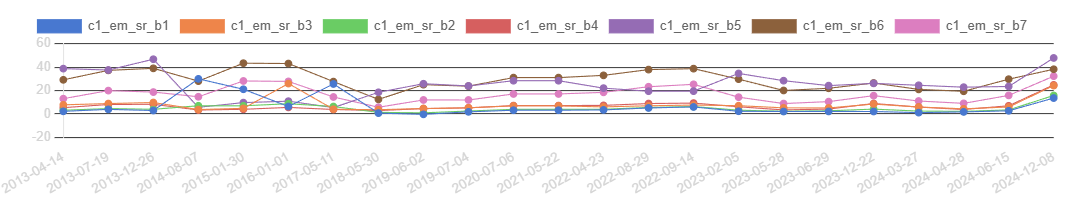
\includegraphics[width=0.97\linewidth]{FIGURAS/pontoC1}
 	\end{center}
 	\begin{center}
 		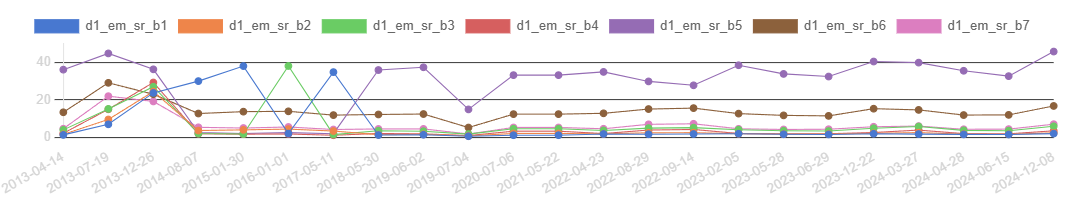
\includegraphics[width=0.97\linewidth]{FIGURAS/PontoD1}
 	\end{center}
 	
 \end{comment}
 
 \subsection{Analise da validação cruzada do Modelo }
 
   \lstset{
 	language=R, % Define a linguagem como R
 	caption= Resultado do Teste Shapiro-Wilk em linguagem R,} % Legenda do código
 \begin{lstlisting}[language=R]
 	Shapiro-Wilk normality test
 	
 	data:  Mod_esfe$pred
 	W = 0.93923, p-value = 1.384e-14
 \end{lstlisting} 
 
   \lstset{
 	language=R, % Define a linguagem como R
 	caption= Resultado do Teste de Correlação em linguagem R,} % Legenda do código
 \begin{lstlisting}[language=R]
 	
 	Pearson's product-moment correlation
 	
 	data:  Mod_esfe$pred and Mod_esfe$observed
 	t = 24.657, df = 574, p-value < 2.2e-16
 	alternative hypothesis: true correlation is not equal to 0
 	95 percent confidence interval:
 	0.6750592 0.7546794
 	sample estimates:
 	cor 
 	0.7172019 
 \end{lstlisting}   
 
% {{{   
		 \begin{minipage}[t!]{0.32\textwidth}
				\begin{figure}[H]
					\centering  \small \caption{Distancia de Cooks e Alavancagem}
					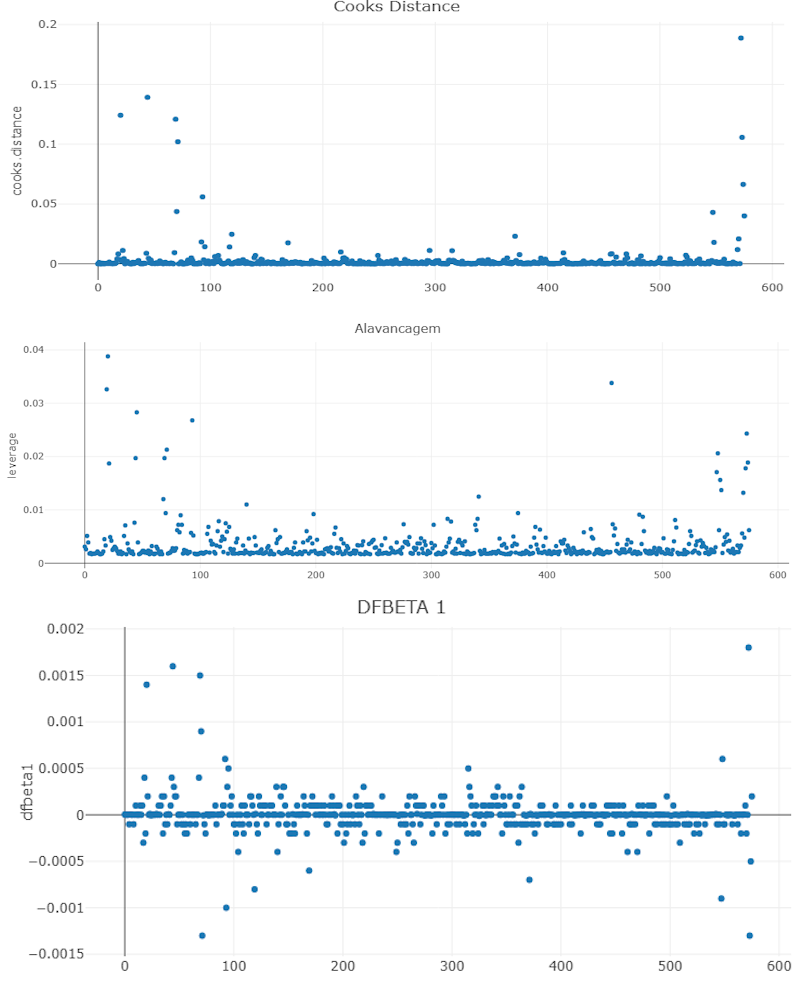
\includegraphics[width=0.97\linewidth]{FIGURAS/dist-cook-alavan}
					\label{fig:DISTCOOK}
				\end{figure}
				
			\end{minipage}\hfill
			\begin{minipage}[t!]{0.332\textwidth}
					\begin{figure}[H]
				    \centering  \small \caption{Analise gráfica da  normalidade}
					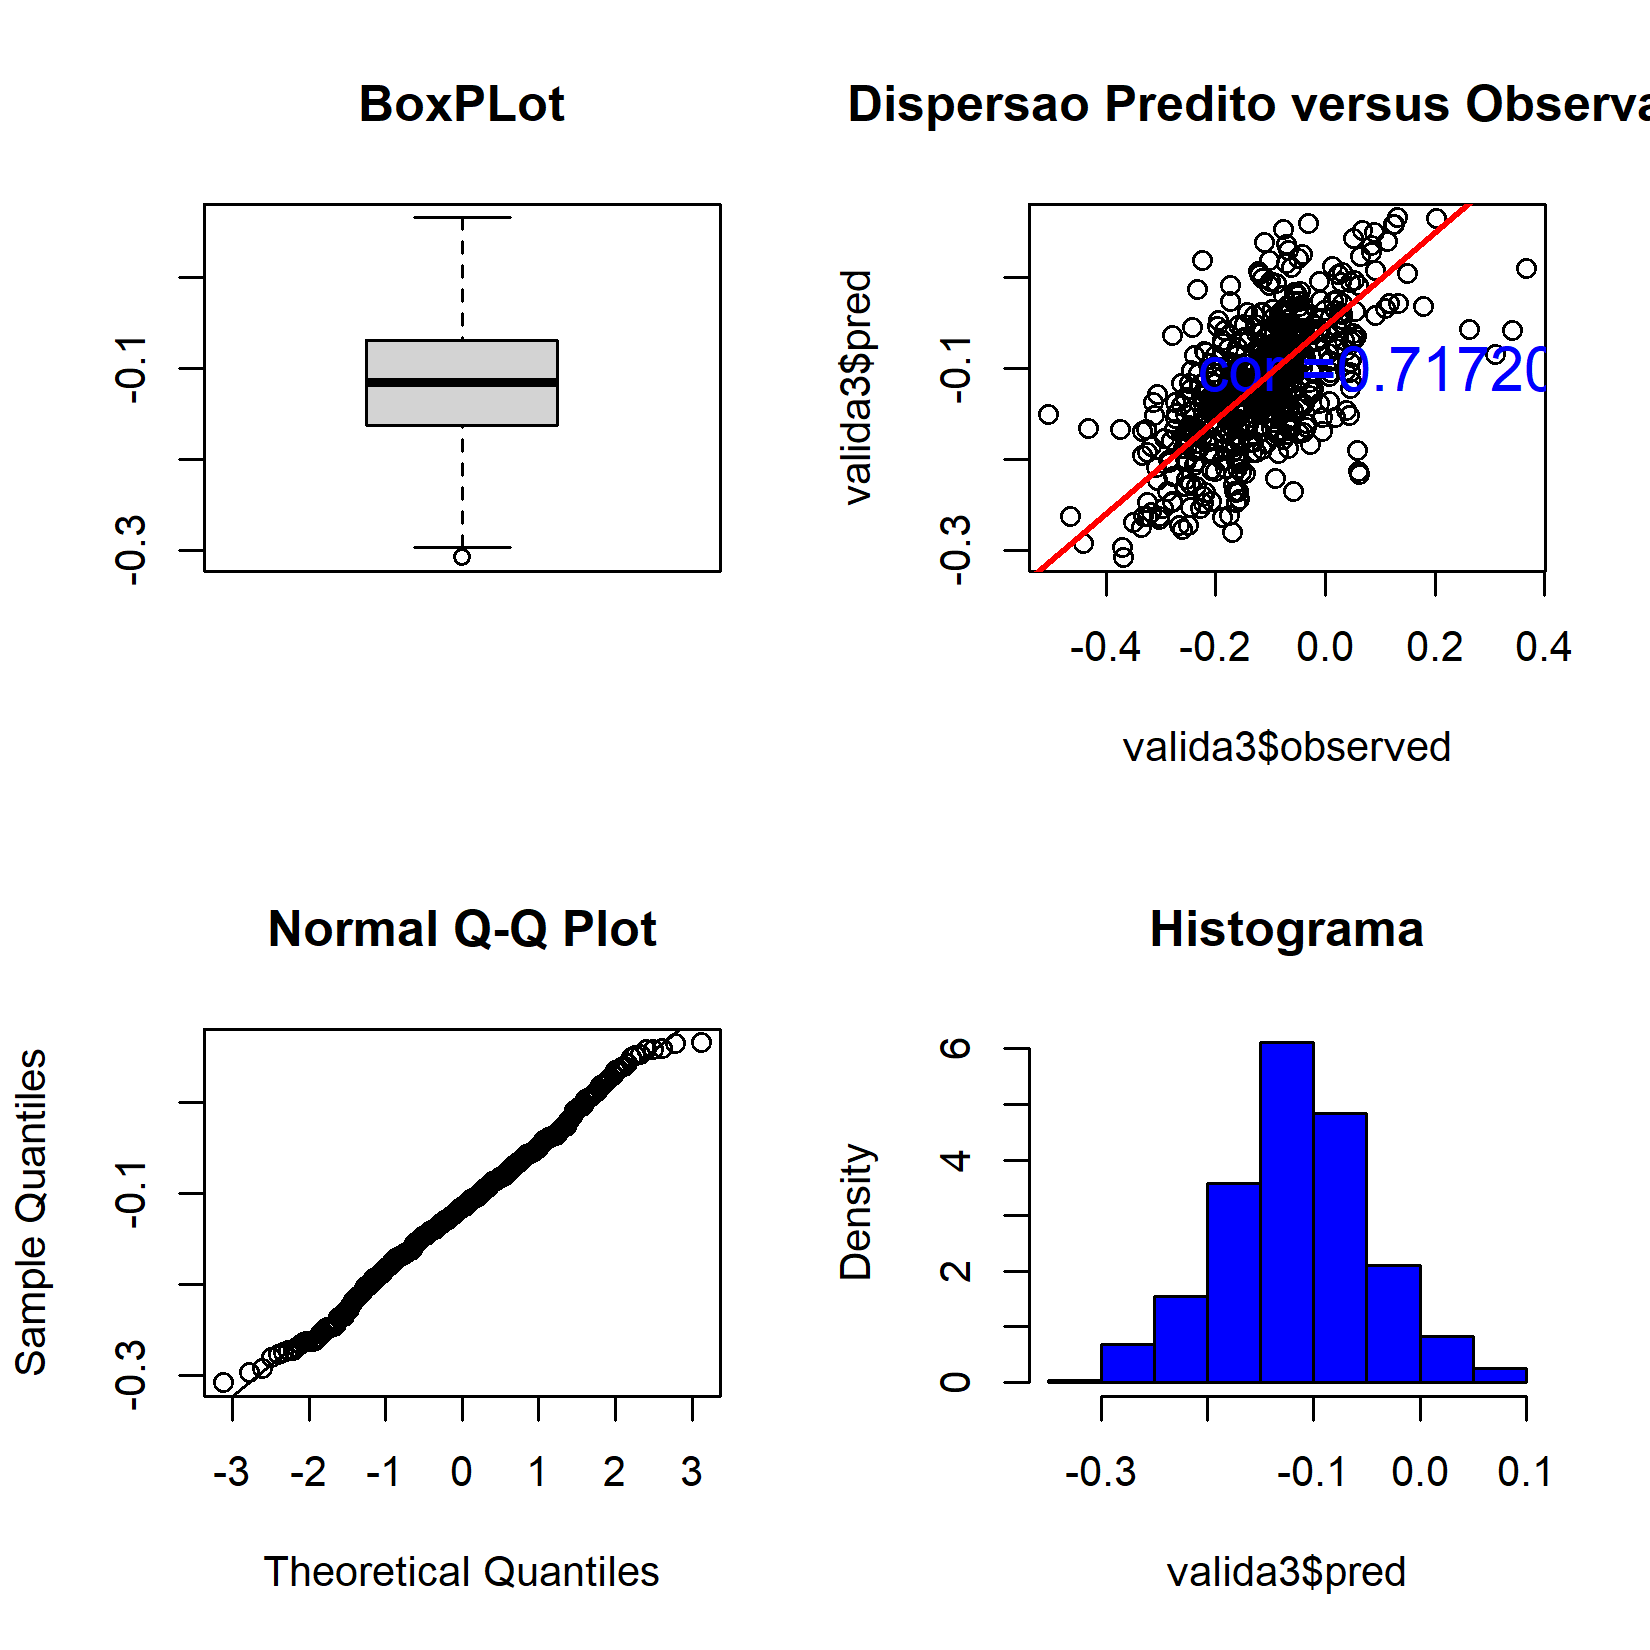
\includegraphics[width=0.97\linewidth]{FIGURAS/valicas}
					\label{fig:valicas}
				\end{figure}
				
			\end{minipage}\hfill
			\begin{minipage}[t!]{0.32\textwidth}
					\begin{figure}[H]
					\centering  \small \caption{Analise gráfica da  correlação entre variáveis}
					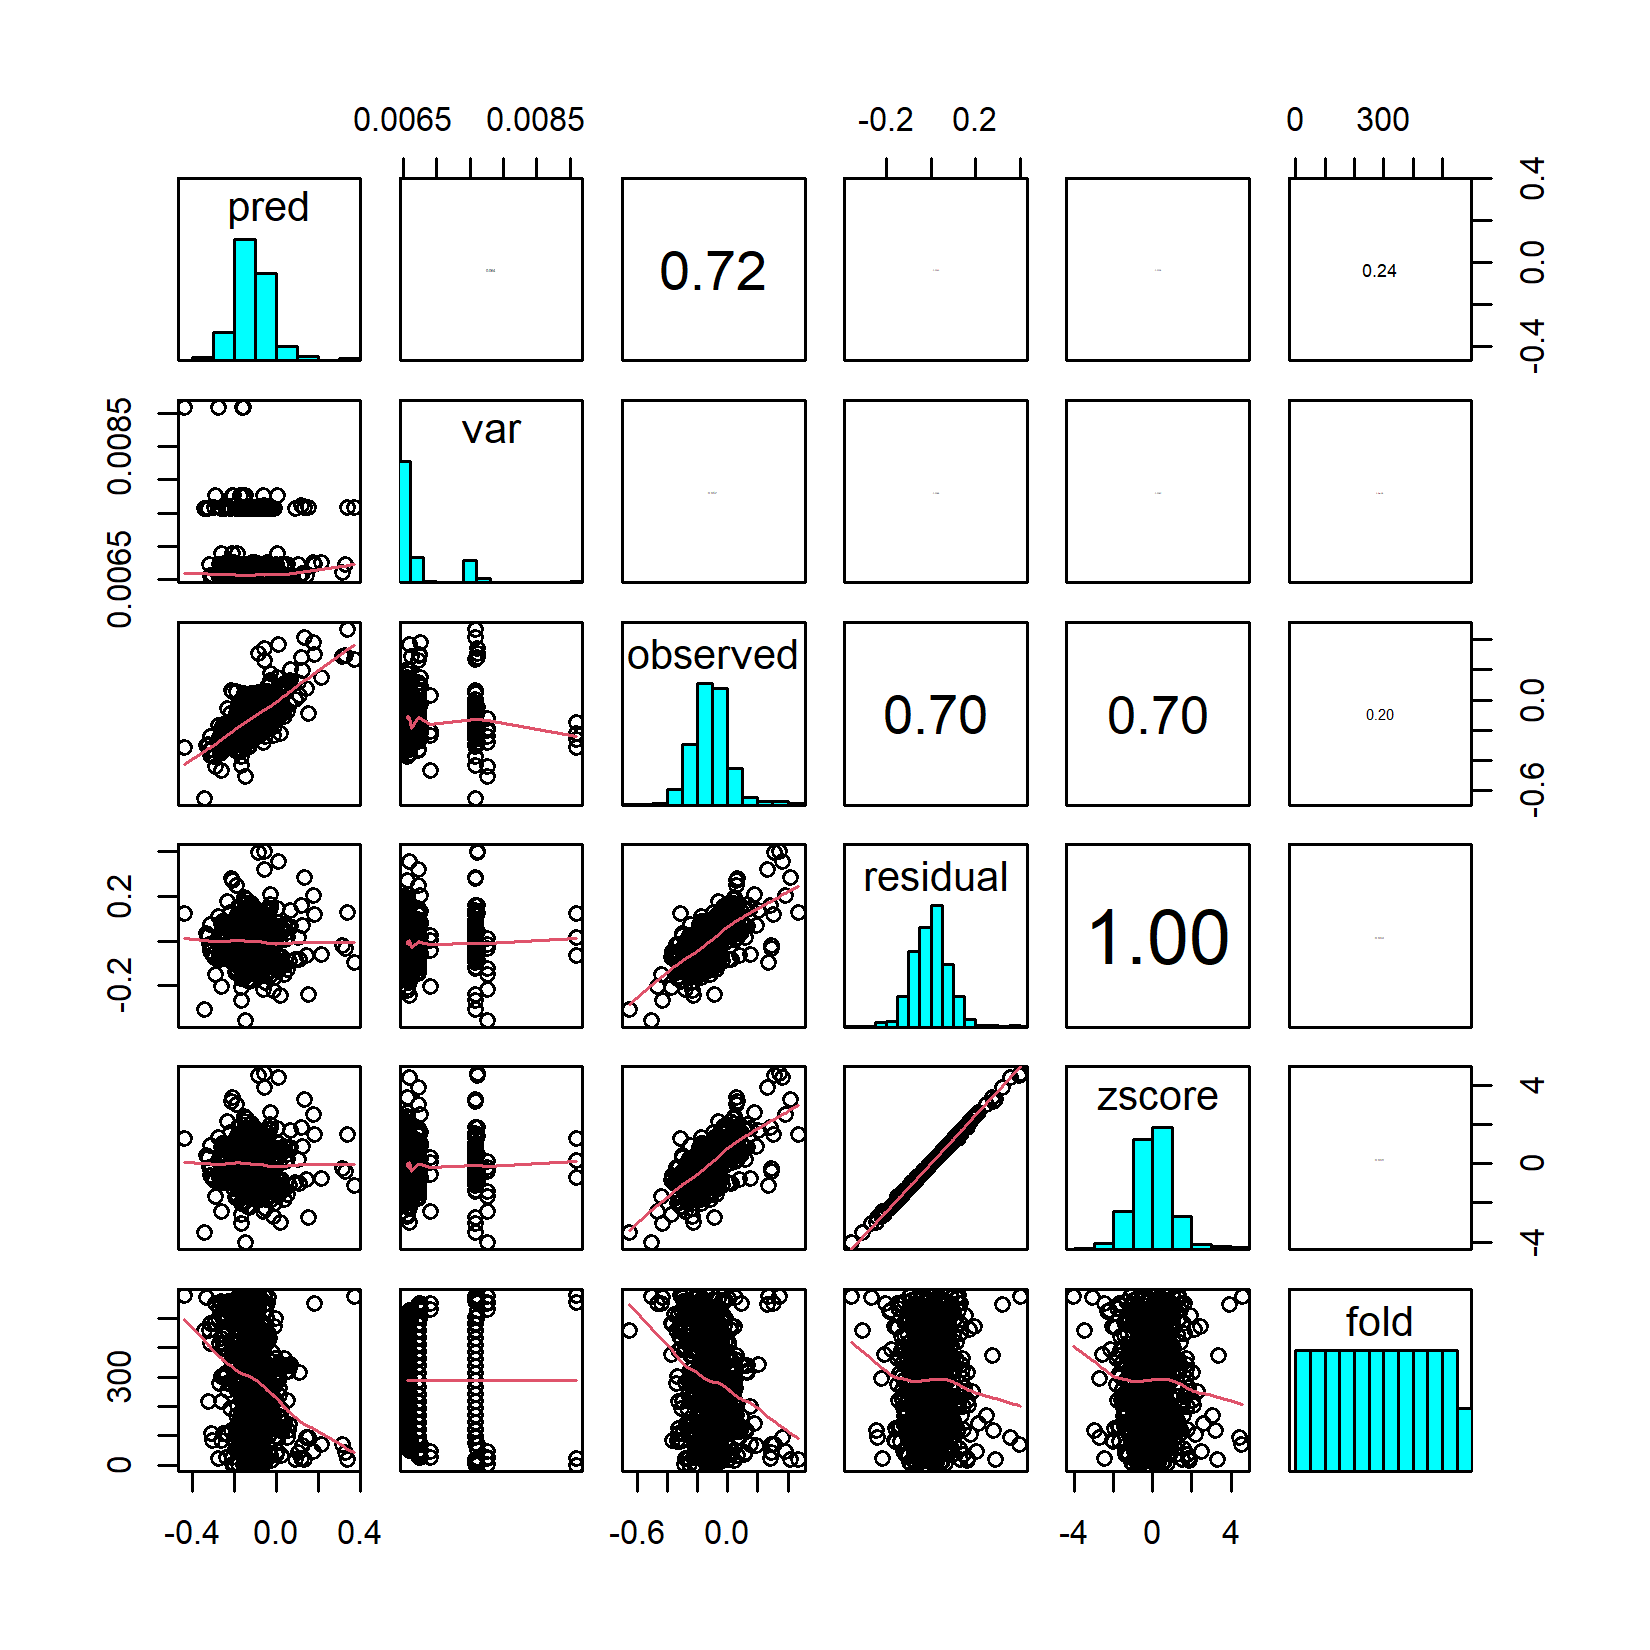
\includegraphics[width=0.7\linewidth]{FIGURAS/painel-correla}
					\label{fig:painel-correla}
				\end{figure}
				
			\end{minipage} 
			 			\begin{center}
				Fonte:   Elaborado pelos Autores (2025)
			\end{center}
			% }}} 
 
 
 
\subsection{Dinâmica temporal }
\hspace*{1.25 cm} E finalmente, passamos para a análise temporal, o qual escolhemos uma posição geográfica onde ocorrem uma maio variação deste modelo superficial de variações de reflectância, pode análise temporal entre as diferenças  \( \Delta T = T_{2}  - T_{1} \)\\
%
\hspace*{1.25 cm}  Na Figura \ref{fig:INDICES}, mostra o comportamento anômalo de todos os índices espectrais ao inicio do ano de 2016, junto a margem.\\

 \begin{figure}[H]
	\centering  \small \caption{Índices em  análise temporal}
	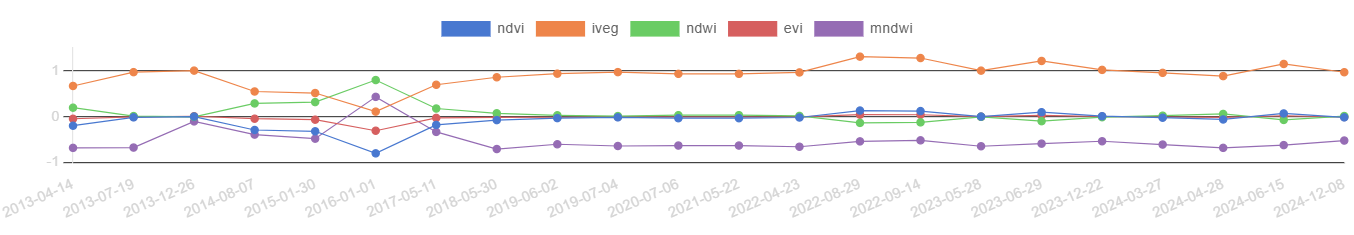
\includegraphics[width=0.97\linewidth]{FIGURAS/indices}
	\label{fig:INDICES}{ Fonte:   Elaborado pelos Autores (2025)}
\end{figure}

 \begin{figure}[H]
	\centering  \small \caption{Aumento do óxido de ferro no período}
	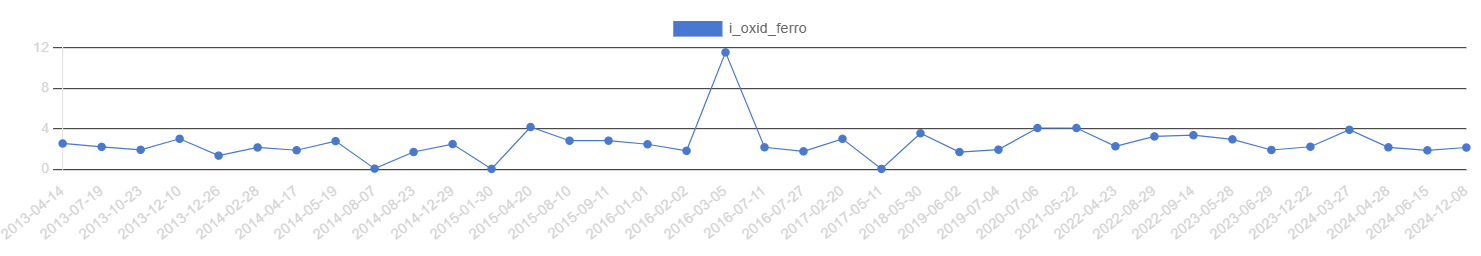
\includegraphics[width=0.97\linewidth]{FIGURAS/graphvisualiser-1747928533564}
	\label{fig:INDICES2}{ Fonte:   Elaborado pelos Autores (2025)}
\end{figure}

\hspace*{1.25 cm} A variação do óxido de ferro alcançou o máximo ao ano de 2018 como Figura \ref{fig:INDICES2}\\
%
\begin{figure}[H]
	\centering  \small \caption{Índices NDVI e NDWI}
	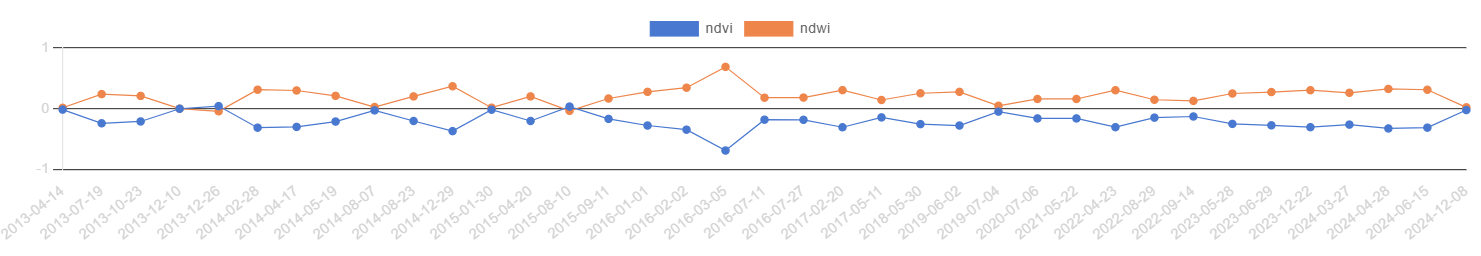
\includegraphics[width=0.97\linewidth]{FIGURAS/graphvisualiser-1747928457345}
	\label{fig:INDICES3}{ Fonte:   Elaborado pelos Autores (2025)}
\end{figure}


